%\documentstyle[12pt]{article}  
\documentclass[12pt]{article}
\usepackage{graphicx}

%% page lay-out  / RUNNING HEAD 
\pagestyle{myheadings} 
\markright{\underline{SPARSKIT \hskip 5.3in} \hskip -1.0in}
\setlength{\headheight}{0.3in} 
\setlength{\headsep}{0.3in}
%% 
\setlength{\textheight}{8.7in} 
\setlength{\textwidth}{6.2in}     
\setlength{\oddsidemargin}{0.2in}  % 
\setlength{\evensidemargin}{0.2in} % 
\setlength{\parindent}{0.2in} %
\setlength{\topmargin}{-0.3in} %%
%% abstract redefinition.
\def\@abssec#1{\vspace{.5in}\footnotesize \parindent 0.2in 
{\bf #1. }\ignorespaces}
\def\abstract{\@abssec{Abstract}}
%%
\setcounter{secnumdepth}{5}
\setcounter{tocdepth}{5}
%%  a few macros 
\def\half{{1\over2}}%
\def\del{\partial} %
\def\nref#1{(\ref{#1})} 
%% more macros: for indented boxes. 
\def\marg#1{\parbox[b]{1.3in}{\bf #1}} 
\def\disp#1{\parbox[t]{4.62in}{#1} \vskip 0.2in } 
%%
%\input{psfig}

\title{
\parbox{4in}{SPARSKIT: a basic tool kit for sparse 
matrix computations } }
\author{\parbox{4in}{VERSION 2\\Youcef Saad\thanks{
Work done partly at CSRD, university of Illinois and partly at RIACS
(NASA Ames Research Center). Current address: Computer Science Dept.,
University of Minnesota, Minneapolis, MN 55455.
This work was supported in part by the NAS Systems 
Division, via Cooperative Agreement NCC 2-387 between NASA and 
the University Space Research Association (USRA)
and in part  by the Department of Energy under grant 
DE-FG02-85ER25001.}}}

\date{ } 

\begin{document}
\bibliographystyle{plain}
%\bibliographystyle{SIAM}

\maketitle

\vskip 1.5in

\centerline{{\it June 6, 1994} } 
%\centerline{{\it May 21, 1990} } 
%\centerline{{\it Updated June 5, 1993 --- Version 2} }  

\thispagestyle{empty}

\begin{abstract} 
This paper presents the main features of a tool package for 
manipulating and working with sparse matrices.
One of the  goals of the package is to provide 
basic tools to facilitate exchange of software and data
between researchers in sparse matrix computations.
Our starting point is the Harwell/Boeing collection of matrices
for which we provide a number of tools. 
Among other things the package provides programs for converting
data structures, printing simple statistics on a matrix, 
plotting a matrix profile, performing  basic linear algebra 
operations  with sparse matrices  and so on.
\end{abstract}

\newpage

\section{Introduction} Research   on   sparse  matrix   techniques  has  become
increasingly complex, and this trend is likely to accentuate if only
because  of the growing need 
to design efficient sparse matrix algorithms for modern supercomputers.   
While there  are a  number of packages and `user
friendly' tools, for  performing computations  with small dense
matrices there is a lack of any similar tool or in fact of any 
general-purpose libraries for 
working with sparse  matrices.   Yet a  collection of  a few  basic programs to
perform some elementary and  common tasks  may be  very useful  in reducing the
typical time to implement and test sparse matrix algorithms.   That a common 
set
of routines  shared  among  researchers  does not  yet exist for sparse matrix
computation is rather surprising.  Consider the contrasting  situation in dense
matrix computations.  The Linpack  and Eispack  packages developed  in the 70's
have been of tremendous  help in  various areas  of scientific  computing.  
One might speculate on the number of hours of programming efforts 
saved worldwide thanks to the widespread availability  of these  packages.
In contrast,  it is  often the case that  researchers in  sparse  matrix 
computation  
code their own subroutine for  such  things as converting the storage mode
of a matrix or for reordering a matrix
according to a certain permutation.  One of the  reasons for this situation
might be the absence of any standard for sparse
matrix computations.  For instance, the number of different data
structures used to store sparse matrices in various applications is
staggering.  For the same basic data structure there often exist a
large number of variations in use.  As sparse matrix computation
technology is maturing there is a desperate need for some standard for
the basic storage schemes and possibly, although this is more
controversial, for the basic linear algebra operations.  

An important example where a package such as SPARSKIT can be helpful is for
exchanging matrices for research or other purposes.  In this
situation, one must often translate the matrix from some initial data
structure in which it is generated, into a different desired data
structure.  One way around this difficulty is to restrict 
the number of schemes that can be used and set  some standards.
 However, this is not
enough because often the data structures are chosen for their
efficiency and convenience, and it is not reasonable to ask
practitioners to abandon their favorite storage schemes.  What is
needed is a large set of programs to translate one data structure into
another. In the same vein, subroutines that generate test matrices
would be extremely valuable since they would allow users to have
access to a large number of matrices without the burden of actually
passing large sets of data.

A useful collection of sparse matrices known as the Harwell/Boeing
collection, which is publically available \cite{Duff-HB}, has been
widely used in recent years for testing and comparison purposes.
Because of the importance of this collection many of the tools in
SPARSKIT can be considered as companion tools to it. For
example, SPARSKIT supplies simple routines to create a Harwell/Boeing (H/B)
file from a matrix in any format, tools for creating pic files in
order to plot a H/B matrix, a few routines that will deliver
statistics for any H/B matrix, etc.. However, SPARSKIT is not limited
to being a set of tools to 
work with H/B matrices. Since one of our main motivations is
research on iterative methods, we provide numerous subroutines that may help
researchers in this specific area.  
SPARSKIT will hopefully be an evolving package
that will benefit from contributions from other researchers. This
report is a succinct description of the  package in this release.

\begin{figure}[h]
%\special{psfile=dir.eps vscale = 75 hscale = 75 hoffset =0 voffset= -30}
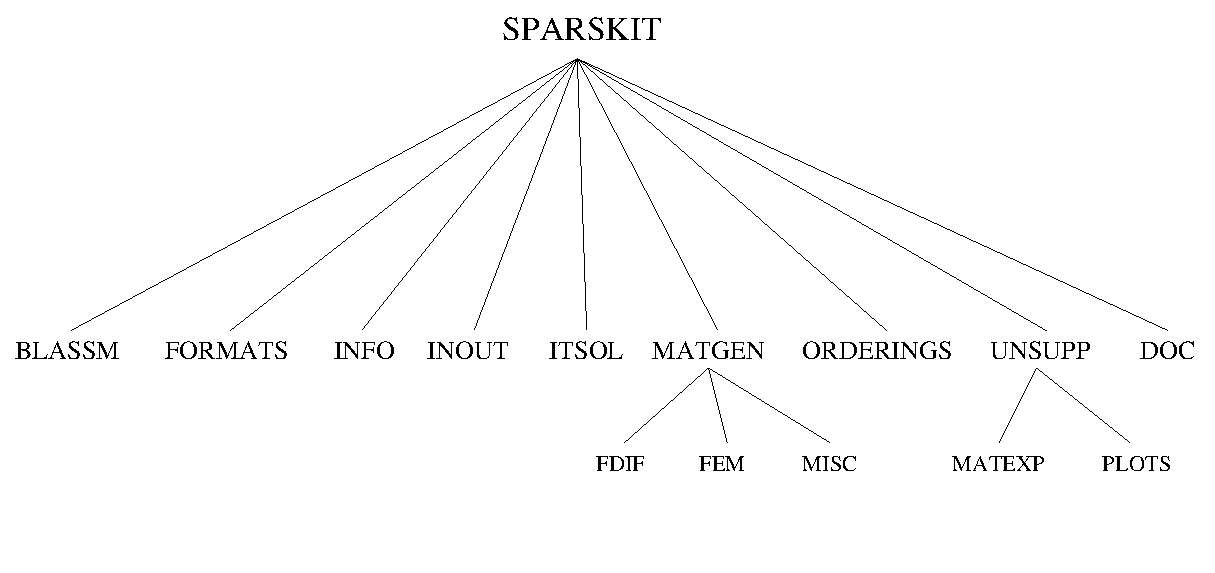
\includegraphics[width=15cm]{dir}
\caption {General organization of SPARSKIT.}
\label{organization}
%\vskip 0.1cm
\end{figure}

\section{Data structures for sparse matrices and the conversion routines}

One of the difficulties in sparse matrix computations is the variety
of types of matrices that are encountered in practical applications.
The purpose of each of these schemes is to gain efficiency both in
terms of memory utilization and arithmetic operations.  As a result
many different ways of storing sparse matrices have been devised to
take advantage of the structure of the matrices or the specificity of
the problem from which they arise.  For example if it is known that a
matrix consists of a few diagonals one may simply store these
diagonals as vectors and the offsets of each diagonal with respect to
the main diagonal.  If the matrix is not regularly structured, then
one of the most common storage schemes in use today is what we refer
to in SPARSKIT as the Compressed Sparse Row (CSR) scheme. In this
scheme all the nonzero entries are stored row by row  in a 
one-dimensional real array $A$ together with an array $JA$ containing
their column indices and a pointer array which contains the addresses
in $A$ and $JA$ of the beginning of each row. The order of the elements 
within each row does not matter. Also of importance
because of its simplicity is the coordinate storage scheme in which
the nonzero entries of $A$ are stored in any order together with their
row and column indices.  Many of the other existing schemes are
specialized to some extent. The reader is
referred to the book by Duff et al. \cite{Duff-book} for more details.

\subsection{Storage Formats} 	
Currently, 
the conversion routines of SPARSKIT can handle thirteen different storage
formats. These include some of the most commonly used schemes but they
are by no means exhaustive.  We found it particularly useful to have
all these storage modes when trying to extract a matrix from someone
else's application code in order, for example, to analyze it with the
tools described in the next sections or, more commonly, to try a given
solution method which requires a different data structure than the
one originally used in the application.  Often the matrix is stored in
one of these modes or a variant that is very close to it.  We hope to
add many more conversion routines as SPARSKIT evolves.

In this section we describe in detail the storage schemes that are
handled in the FORMATS module.  For convenience we have decided to
label by a three character name each format used.  We start by listing
the formats and then describe them in detail  in separate subsections
(except for the dense format which needs no detailed description).	

\begin{description}
\item{{\bf DNS}} Dense format
\item{{\bf BND}} Linpack Banded format
\item{{\bf CSR}} Compressed Sparse Row format 
\item{{\bf CSC}} Compressed Sparse Column format 
\item{{\bf COO}} Coordinate format
\item{{\bf ELL}} Ellpack-Itpack generalized diagonal format
\item{{\bf DIA}} Diagonal format
\item{{\bf BSR}} Block Sparse Row format
\item{{\bf MSR}} Modified Compressed Sparse Row format
\item{{\bf SSK}} Symmetric Skyline format
\item{{\bf NSK}} Nonsymmetric Skyline format
\item{{\bf LNK}} Linked list storage format 
\item{{\bf JAD}} The Jagged Diagonal format 
\item{{\bf SSS}} The Symmetric Sparse Skyline format
\item{{\bf USS}} The Unsymmetric Sparse Skyline format
\item{{\bf VBR}} Variable Block Row format
\end{description}

In the following sections we denote by $A$ the matrix under
consideration and by $N$ its row dimension and $NNZ$ the number of its
nonzero elements.

\subsubsection{Compressed Sparse Row and related formats
 (CSR, CSC and MSR)} The Compressed Sparse Row format is the basic
format used in SPARSKIT. Its  data structure consists of three arrays.

\begin{itemize} 

\item A real array $A$ containing the real values $a_{ij}$ stored row by row,
from row 1 to $N$. The length of $A$ is NNZ.

\item An integer array $JA$ containing the column indices
of the elements $a_{ij}$ as stored in the array $A$.  The length of
$JA$ is NNZ.

\item An integer array $IA$ containing the pointers to the
beginning of each row in the arrays $A$ and $JA$. Thus the content of
$IA(i)$ is the position in arrays $A$ and $JA$ where the $i$-th row
starts.  The length of $IA$ is $N+1$ with $IA(N+1)$ containing the
number $IA(1)+NNZ$, i.e., the address in $A$ and $JA$ of the beginning
of a fictitious row $N+1$.

\end{itemize}
The order of the nonzero elements within the same row are not important. 
A variation to this scheme is to sort the elements in each row 
in such a way that their column positions are in increasing order.
When this sorting in enforced, it is often possible to 
make substantial savings in the number of operations of 
some well-known algorithms. 
The Compressed Sparse Column format is identical with the Compressed
Sparse Row format except that the columns of $A$ are stored instead of
the rows. In other words the Compressed Sparse Column format is simply
the Compressed Sparse Row format for the matrix $A^T$.

The Modified Sparse Row (MSR) format is a rather common variation of
the Compressed Sparse Row format which consists of keeping the main
diagonal of $A$ separately. The corresponding data structure consists
of a real array $A$ and an integer array $JA$. The first $N$ positions
in $A$ contain the diagonal elements of the matrix, in order.  The position
$N+1$ of the array $A$ is not used. Starting from position $N+2$, the
nonzero elements of $A$, excluding its diagonal elements, are stored
row-wise. Corresponding to each element $A(k)$ the integer $JA(k)$ is
the column index of the element $A(k)$ in the matrix $A$. The $N+1$
first positions of $JA$ contain the pointer to the beginning of each
row in $A$ and $JA$. The advantage of this storage mode is that many
matrices have a full main diagonal, i.e., $a_{ii} \ne 0, i=1,\ldots,
N$, and this diagonal is best represented by an array of length $N$.
This storage mode is particularly useful for triangular matrices with
non-unit diagonals. Often the diagonal is then stored in inverted form
(i.e. $1/a_{ii} $ is stored in place of $a_{ii} $) because triangular
systems are often solved repeatedly with the same matrix many times,
as is the case for example in preconditioned Conjugate Gradient
methods.  The column oriented analogue of the MSR format, called MSC
format, is also used in some of the other modules, but no
transformation to/from it to the CSC format is necessary: for example
to pass from CSC to MSC one can use the routine to pass from the CSR
to the MSR formats, since the data structures are identical.  The 
 above three storage modes are used in many well-known packages.

\subsubsection{The banded Linpack format (BND)} 
Banded matrices represent the simplest form of sparse matrices and
they often convey the easiest way of exploiting sparsity.  There are
many ways of storing a banded matrix. The one we adopted here follows
the data structure used in the Linpack banded solution routines. Our
motivation is that one can easily take advantage of this widely available 
package if the matrices are banded.  For fairly small matrices (say,
$N < 2000$ on supercomputers, $ N < 200 $ on fast workstations, and
with a bandwidth of $O(N^{\half} )$), this may represent a viable and
simple way of solving linear systems. One must first transform the
initial data structure into the banded Linpack format and then call the
appropriate band solver. For large problems it is clear that a better
alternative would be to use a sparse solver such as MA28, which
requires the input matrix to be in the coordinate format. 

%%It is
%%expected that these types of utilization of the conversion routines
%% will in fact be among the most common ones.

In the BND format the nonzero elements of $A$ are stored in a
rectangular array $ABD$ with the nonzero elements of the $j$-th column
being stored in the $j-th$ column of $ABD$. We also need to know the
number $ML$ of diagonals below the main diagonals and the number $MU$
of diagonals above the main diagonals. Thus the bandwidth of $A$ is
$ML+MU+1$ which is the minimum number of rows required in the array
$ABD$. An additional integer parameter is needed to indicate which row
of $ABD$ contains the lowest diagonal.

\subsubsection{The coordinate format (COO) } 

The coordinate format is certainly the simplest storage scheme for
sparse matrices. It consists of three arrays: a real array of size
$NNZ$ containing the real values of nonzero elements of $A$ in any
order, an integer array containing their row indices and a second
integer array containing their column indices. Note that this scheme
is as general as the CSR format, but from the point of view of memory
requirement it is not as efficient.  On the other hand it is
attractive because of its simplicity and the fact that it is very
commonly used.  Incidentally, we should mention a variation to this
mode which is perhaps the most economical in terms of memory usage.
The modified version requires only a real array $A$ containing the
real values $a_{ij}$ along with only one integer array that contains
the integer values $ (i-1)N + j$ for each corresponding nonzero
element $a_{ij}$.  It is clear that this is an unambiguous
representation of all the nonzero elements of $A$.  There are two
drawbacks to this scheme. First, it requires some integer arithmetic
to extract the column and row indices of each element when they are
needed. Second, for large matrices it may lead to integer overflow
because of the need to deal with integers which may be very large (of
the order of $N^2$).  Because of these two drawbacks this scheme has
seldom been used in practice.

\subsubsection{The diagonal format (DIA) }
The matrices that arise in many applications often consist of a few
diagonals. This structure has probably been the first one to be
exploited for the purpose of improving performance of
matrix by vector products on supercomputers, see references in
\cite{Saad-Boeing}.  To store
these matrices we may store the diagonals in a rectangular array
$DIAG(1:N,1:NDIAG) $ where $NDIAG$ is the number of diagonals.  We
also need to know the offsets of each of the diagonals with respect to
the main diagonal. These will be stored in an array $IOFF(1:NDIAG)$.
Thus, in position $(i,k)$ of the array $DIAG$ is located the element
$a_{i,i+ioff(k)}$ of the original matrix.  The order in which the
diagonals are stored in the columns of $DIAG$ is unimportant.  Note
also that all the diagonals except the main diagonal have fewer than
$N$ elements, so there are positions in $DIAG$ that will not be used.

In many applications there is a small number of non-empty diagonals
and this scheme is enough. In general however, it may be desirable to
supplement this data structure, e.g., by a compressed sparse row
format.  A general matrix is therefore represented as the sum of a
diagonal-structured matrix and a general sparse matrix.  The
conversion routine CSRDIA which converts from the compressed
sparse row format to the diagonal format has an option	 to this
effect.  If the user wants to convert a general sparse matrix to one
with, say, 5 diagonals, and if the input matrix has more than 5
diagonals, the rest of the matrix (after extraction of the 5 desired
diagonals) will be put, if desired, into a matrix in the CSR format.
In addition, the code may also compute the most important 5 diagonals
if wanted, or it can get those indicated by the user through the array
$IOFF$.

\subsubsection{The Ellpack-Itpack format (ELL) }
The Ellpack-Itpack format
\cite{Oppe-Kincaid,Young-Oppe-al,Oppe-NSPCG} is a 
generalization of the diagonal storage scheme which is intended for
general sparse matrices with a limited maximum number of nonzeros per
row. Two rectangular arrays of the same size are required, one real
and one integer.  The first, $COEF$, is similar to $DIAG$ and contains
the nonzero elements of $A$. Assuming that there are at most $NDIAG$
nonzero elements in each row of $A$, we can store the nonzero elements
of each row of the matrix in a row of the array $COEF(1:N,1:NDIAG)$
completing the row by zeros if necessary.  Together with $COEF$ we
need to store an integer array $JCOEF(1:N,1:NDIAG)$ which contains the
column positions of each entry in $COEF$.

\subsubsection{The Block Sparse Row format (BSR)} 
Block matrices are common in all areas of scientific computing. The
best way to describe block matrices is by viewing them as sparse
matrices whose nonzero entries are square dense blocks. Block matrices
arise from the discretization of partial differential equations when
there are several degrees of freedom per grid point.  There are
restrictions to this scheme. Each of the blocks is treated as a dense
block. If there are zero elements within each block they must be
treated as nonzero elements with the value zero.

There are several variations to the method used for storing sparse
matrices with block structure. The one considered here, the Block
Sparse Row format, is a simple generalization of the Compressed Sparse
Row format.

We denote here by $NBLK$ the dimension of each block, by 
$NNZR$ the number of nonzero blocks in $A$ (i.e., 
$NNZR = NNZ/(NBLK^2) $) and by $NR$ the block dimension of $A$,
(i.e., $NR = N/NBLK$), the letter $R$ standing for `reduced'. 
Like the Compressed Sparse Row  format we need three arrays. A rectangular
real array $A(1:NNZR,1:NBLK,1:NBLK) $ contains the nonzero
blocks listed (block)-row-wise. Associated with this real array
is an integer array 
$JA(1:NNZR) $ which holds the actual column positions in the 
original matrix of the $(1,1)$ elements of the nonzero blocks.
Finally, the pointer array $IA(1:NR+1)$ points to the beginning
of each block row in $A$ and $JA$. 

The savings in memory and in the use of indirect addressing with  this
scheme over Compressed Sparse Row   can be substantial for large
values of $NBLK$.

\subsubsection{The Symmetric Skyline format (SSK) }
A skyline matrix is often referred to as a variable band
matrix or a profile matrix \cite{Duff-book}.  The main 
attraction of skyline matrices is that when pivoting is
not necessary then the skyline structure of the matrix is preserved 
during Gaussian elimination. If the matrix is symmetric
we only need to store its lower triangular part. This is a
collection of rows whose length varies. A simple method used to store
a Symmetric Skyline matrix is to place all the rows in order from
1 to $N$ in a  real array $A$ and then keep an integer array which holds 
the pointers to the beginning of each row, see \cite{Duff-survey}.
The column positions of the nonzero elements stored in $A$
can easily be derived and are therefore not needed. However, there 
are several variations to this scheme that are commonly used is
commercial software packages. For example, we found that in many 
instances the pointer is to the diagonal element rather than to the 
first element in the row. In some cases (e.g., IBM's ISSL library)
both are supported. Given that these variations are commonly used 
it is a good idea to provide at least a few of them. 

\subsubsection{The Non Symmetric Skyline format (NSK) }
Conceptually, the  data structure of a nonsymmetric skyline 
matrix consists of two substructures. 
The first consists of the lower part of $A$ stored in skyline format
and the second of its upper triangular part stored in a column
oriented skyline format (i.e., the transpose is stored in
standard row skyline mode). Several ways of putting these
substructures together may be used and there are no compelling 
reasons for preferring one strategy over another one. 
One possibility is to use two separate arrays $AL$ and $AU$ for
the lower part and upper part respectively, with the diagonal 
element in the upper part. The data structures for each of 
two parts is similar to that used for the SSK storage.

%% NOT DONE YET --- 
%%We chose to store contiguously each row of the lower part and column of 
%%the upper part of the matrix.  The real array $A$ will contain 
%%the 1-st row followed by the first column (empty), followed
%%by the second row followed by the second column, etc..
%%An additional pointer is needed to indicate where the
%%diagonal elements, which separate the lower from the upper part,
%%are located in this array. G

\subsubsection{The linked list storage format (LNK) }  
This is one of the oldest data structures used for sparse matrix computations.
It consists of four arrays: $A$, $JCOL$, $LINK$ and $JSTART$. 
The arrays $A$ and $JCOL$ contain the nonzero elements and their
corresponding column indices respectively. The integer array $LINK$ is
the usual link pointer array in linked list data structures: 
$LINK(k)$ points to the position of the nonzero element next to 
$A(k), JCOL(k)$ in the same row. Note that the order of the elements 
within each row is unimportant.  If $LINK(k) =0$ then there is no
next element, i.e., $A(k), JCOL(k)$ is the last element of the row.
Finally, $ISTART$ points to the first element of each row in 
in the previous arrays. Thus, $k=ISTART(1)$ points to the first element
of the first row, in $A, ICOL$, 
 $ISTART(2) $ to the second element, etc..
As a convention $ISTART(i) = 0$, means that the $i$-th row is empty.

\subsubsection{The Jagged Diagonal format (JAD)} 
This storage mode is very useful for the efficient implementation
of iterative methods on  parallel and vector processors
\cite{Saad-Boeing}. Starting from the CSR format, the idea is to 
first reorder the rows of the matrix decreasingly according to their 
number of nonzeros entries. Then, a new data structure is built 
by constructing what we call ``jagged diagonals" (j-diagonals).
We store as a dense vector, the vector consisting of all
the first elements in $A, JA$ from each row, together with an integer 
vector containing the column positions of the corresponding 
elements. This is followed by the second jagged  diagonal consisting of the
elements in the second positions from the left. As we build more and
more of these diagonals, their length decreases.  The number of
j-diagonals is equal to the number of nonzero elements of the first
row, i.e., to the largest number of nonzero elements per row.  The
data structure to represent a general matrix in this form consists,
before anything, of the permutation array which reorders the rows.
Then the real array $A$ containing the jagged diagonals in succession
and the array $JA$ of the corresponding column positions are stored,
together with a pointer array $ IA $ which points to the beginning of
each jagged diagonal in the arrays $A, JA$. The advantage of this
scheme for matrix multiplications has been illustrated in
\cite{Saad-Boeing} and in \cite{Anderson-Saad} in the 
context of triangular system solutions.

\subsubsection{The Symmetric and Unsymmetric Sparse Skyline format
(SSS, USS)} 

This is an extension of the CSR-type format described above.
In the symmetric version, the following arrays are used:
$DIAG$ stores the diagonal,
$AL, JAL, IAL$ stores the strict lower part in CSR format, and
$AU$ stores the values of the strict upper part in CSC format.
In the unsymmetric version, instead of $AU$ alone, the strict upper part
is stored in $AU, JAU, IAU$ in CSC format.

%% THIS SECTION HAS BEEN MODIFIED
%% \subsubsection{The Compressed Variable Block Format(CVB)}
%% This is an extension of the Block Sparse Row format (BSR). In the BSR
%% format, all the  blocks have the same size.
%% A more general way of partitioning might allow the
%% matrix to be split into different size blocks. In the CVB format, an
%% arbitrary partitioning of the matrix is allowed. However, the columns and
%% the rows must be split in the same way. 
%%
%% Figure 0 shows a 9x9 sparse matrix and its corresponding storage vectors.
%% Let $h$ be the index of the leading elements of the $k^{th}$ block 
%% stored in $AA$. Then $k^{th}$ block of size $m*p$ is stored in  
%% $AA(h)$ to $AA(h+mp-1)$.
%% For  example, the $3^{rd}$ block is stored in $AA(9)$ to $AA(17)$.
%%
%% The data structure consists of the integers \(N\), \(NB\), and the arrays 
%% \(AA\), \(JA\), \(IA\), and
%% \(KVST\), where \(N\) is the matrix size, i.e.~number of rows in the
%% matrix, \(NB\) is the number of block rows, \(AA\) stores the non-zero
%% values of the matrix, \(JA\) has the column indices of the first
%% elements in the blocks, \(IA\) contains the pointers to the beginning
%% of each block row (in \(AA\)), \(KVST\) contains the index of
%% the first row in each block row.
%%
%% \begin{figure}[h]
%% \vspace{3in}
%% \special{psfile= fig1.eps vscale = 100 hscale = 100 hoffset =-50 voffset= -420}
%%\caption {\bf Fig 1: An example of a 9x9 sparse matrix and its storage vectors.  }
%%\label{conventional}
%% \end{figure}

\subsubsection{The Variable Block Row format (VBR)}
In many applications, matrices are blocked, but the blocks are not all
the same size.  These so-called variable block matrices arise from the
discretization of systems of partial differential equations where there
is a varying number of equations at each grid point.  Like in the Block
Sparse Row (BSR) format, all entries of nonzero blocks (blocks which
contain any nonzeros) are stored, even if their value is zero.  Also
like the BSR format, there is significant savings in integer pointer
overhead in the data structure.

Variable block generalizations can be made to many matrix storage
formats.  The Variable Block Row (VBR) format is a generalization of the
Compressed Sparse Row (CSR) format, and is similar to the variable
block format used at the University of Waterloo, and one currently
proposed in the Sparse BLAS toolkit.

In the VBR format, the $IA$ and $JA$ arrays of the CSR format store the
sparsity structure of the blocks.  The entries in each block are stored
in $A$ in column-major order so that each block may be passed as a small
dense matrix to a Fortran subprogram.  The block row and block column
partitionings are stored in the vectors {\em KVSTR} and {\em KVSTC},
by storing the first row or column number of each block row or column
respectively.  In most applications, the block row and column partitionings
will be conformal, and the same array may be used in the programs.
Finally, integer pointers to the beginning of each block in $A$ are stored
in the array $KA$.

$IA$ contains pointers to the beginning of each block row in $JA$ and $KA$.
Thus $IA$ has length equal to the number of block rows (plus one to mark
the end of the matrix), and $JA$ has length equal to the number of nonzero
blocks.  $KA$ has the same length as $JA$ plus one to mark the end of
the matrix.  {\em KVSTR} and {\em KVSTC} have length equal to the number
of block rows and columns respectively, and $A$ has length equal to the
number of nonzeros in the matrix.  The following
figure shows the VBR format applied to a small matrix.

This version of Sparskit has a number of routines to support the variable
block matrix format.  CSRVBR and VBRCSR convert between the VBR and CSR
formats; VBRINFO prints some elementary information about the block
structure of a matrix in VBR format; AMUXV performs a matrix-vector product
with a matrix in VBR format; CSRKVSTR and CSRKVSTC are used
to determine row and column block partitionings of a matrix in CSR format,
and KVSTMERGE is used to combine row and column partitionings to achieve
a conformal partitioning.

\begin{figure}[htb]
%\vspace{4.8in}
%\centerline{\psfig{figure=vbrpic.eps,width=6.2in}}
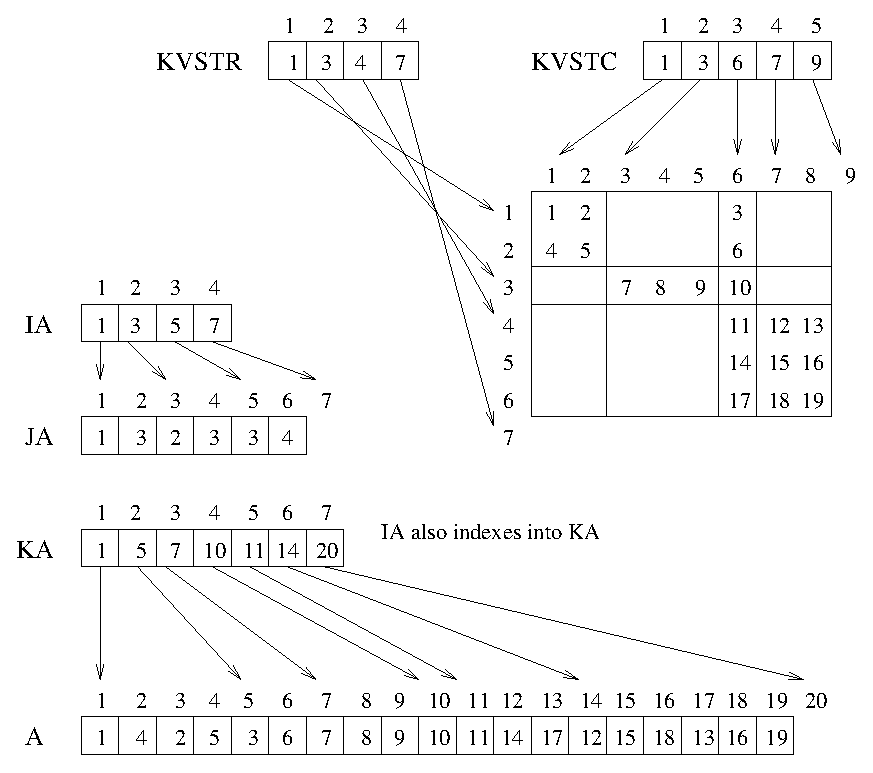
\includegraphics[width=6.2in]{vbrpic}
%\special{psfile=vbrpic.eps vscale = 100 hscale = 100}
%\special{psfile=vbrpic.eps vscale = 100 hscale = 100 voffset= -420}
\caption {A $6 \times 8$ sparse matrix and its storage vectors.}
\end{figure}

\subsection{The FORMATS conversion module}
It is important to note that there is no need to have a subroutine for
each pair of data structures, since all we need is to be able to
convert any format to the standard row-compressed format and then back
to any other format.  There are currently 32 different conversion
routines in this module all of which are devoted to converting from
one data structure into another.

The naming mechanism adopted is to use a 6-character name for each of
the subroutines, the first 3 for the input format and the last 3 for
the output format.  Thus COOCSR performs the conversion from the
coordinate format to the Compressed Sparse Row format.  However it was
necessary to break the naming rule in one exception.  We needed a
version of COOCSR that is in-place, i.e., which can take the input
matrix, and convert it directly into a CSR format by using very little
additional work space.  This routine is called COICSR.  Each of
the formats has a routine to translate it to the CSR format and a routine
to convert back to it from the CSR format.  The only exception is that
a CSCCSR routine is not necessary since
the conversion from Column Sparse format to Sparse Row format  can be
performed with the same routine CSRCSC.  This is essentially a transposition
operation.

Considerable effort has been put at attempting to make the conversion
routines in-place, i.e., in allowing some or all of 
the output arrays to be the same as the input arrays. 
The purpose is to save storage whenever possible without
sacrificing performance. The added flexibility can be 
very convenient in some situations. 
When the additional coding complexity to  permit
the routine to be in-place was not too high this was always done.
If the subroutine is in-place this is clearly indicated in the
documentation. As mentioned above, we found it necessary in one instance
to provide both the in-place version as well as the regular version:
 COICSR is an in-place version of the COOCSR routine.
We would also like to add that other routines that avoid the
CSR format for some of the more important data structures may
eventually be included. For now, there is only one such routine
\footnote{Contributed by E. Rothman from Cornell University.}
namely, COOELL. 

\subsection{Internal format used in SPARSKIT}
Most of the routines in SPARSKIT  use internally the Compressed
Sparse Row format. The selection of 
the CSR mode has been motivated by several factors. Simplicity,
generality, and widespread use are certainly the most 
important ones. However, it has often been argued 
that the column scheme may
have been a better choice. One argument in this favor is that
vector machines usually give a better performance for such 
operations as matrix vector by multiplications for matrices
stored in CSC format. In fact for parallel machines which
have a low overhead in loop synchronization (e.g., the Alliants),
the situation is reversed, see \cite{Saad-Boeing} for details.
For almost any argument in favor of one scheme there seems
to be an argument in favor of the other. Fortunately,
the difference provided in functionality is rather minor.
For example the subroutine APLB to add two matrices in CSR format,
described in Section 5.1, can actually be also used to add 
two matrices in CSC format, since the data structures
are identical. Several such subroutines can be used for both
schemes, by pretending that the input matrices
are stored in CSR mode whereas in fact they are 
stored in CSC mode. 

\section{Manipulation routines} The module UNARY   
of SPARSKIT consists of a  number of  utilities to  manipulate and perform
basic operations with sparse matrices. The  following sections 
give an overview of this part of the package.

\subsection{Miscellaneous operations with sparse matrices}
There are a large number of non-algebraic operations that
are commonly used when working with sparse matrices. 
A typical example is to transform $A$ into $B = P A Q $
where $P$ and $Q$ are two permutation matrices. 
Another example is to extract the lower triangular
part of $A$ or a given diagonal from $A$. Several other 
such `extraction' operations are supplied in SPARSKIT. 
Also provided is the transposition function. This may seem
as an unnecessary addition since the routine 
CSRCSC already does perform this function economically. However,
the new transposition provided is in-place, in that it may
transpose the matrix and overwrite the result on the original matrix,
thus saving memory usage. Since many of these manipulation routines
involve one matrix (as opposed to two in the basic linear algebra routines)
we created a module called  UNARY to include these subroutines.

Another set of subroutines that are sometimes useful 
are those involving  a `mask'. A mask
defines a given nonzero pattern and for all practical
purposes a mask matrix is a sparse matrix whose nonzero
entries are all ones (therefore there is no need to store 
its real values).  Sometimes it is useful
to extract from a given matrix $A$ the `masked' matrix according
to a mask $M$, i.e., to compute the matrix
$A \odot M$ , where $\odot $ denotes the element-wise matrix
product, and $M$ is some mask matrix.

\subsection{The module UNARY}
This module of SPARSKIT consists of a number of routines
to  perform some basic non-algebraic operations on a matrix.
The following is a list of the routines currently supported with
a brief explanation. 
%%There are many other routines which are not 
%% listed their inclusion still being debated.

\vskip .5in

\marg{SUBMAT}\disp{Extracts a square or
rectangular submatrix from a sparse matrix. Both the 
input and output  matrices are in CSR format.
The routine is in-place.} 

\marg{FILTER}\disp{Filters out elements from a
 matrix according to their magnitude. Both the input and
the output matrices are in CSR format.
The output matrix, is obtained from the
input matrix by removing all the elements that are smaller than
a  certain threshold. The threshold is computed for each row
according to one of three provided options.
The algorithm is in-place.}

\marg{FILTERM}\disp{Same as above, but for the MSR format.}

\marg{CSORT}\disp{Sorts the elements of a matrix stored in
CSR format in increasing order of the column numbers. }

\marg{ TRANSP  }\disp{ This is an in-place transposition routine,
i.e., it can be viewed as an in-place version of the CSRCSC 
routine in FORMATS.
One notable disadvantage of  TRANSP is that unlike CSRCSC it 
does not sort the
nonzero elements in increasing number of the column positions.} 

\marg{ COPMAT  }\disp{Copy of a matrix into another 
matrix (both stored CSR).}

\marg{MSRCOP}\disp{Copies a matrix in MSR format into a matrix in MSR format.}
\marg{ GETELM }\disp{Function returning 
the value of $a_{ij}$ for any pair $(i,j)$. Also returns address
of the element in arrays $A, JA$. }

\marg{ GETDIA  }\disp{ Extracts a specified diagonal from a matrix.
An option is provided to transform the input matrix so that the 
extracted diagonal is zeroed out in input matrix. Otherwise the diagonal 
is extracted and the input matrix remains untouched.}

\marg{ GETL    }\disp{This subroutine extracts the
lower triangular part of a matrix, including the main diagonal.
The algorithm is in-place.}

\marg{ GETU    }\disp{Extracts the upper triangular part of
a matrix. Similar to GETL.}

\marg{ LEVELS  }\disp{ 
Computes the level scheduling data structure for lower
triangular matrices, see \cite{Anderson-Saad}.} 

\marg{ AMASK   }\disp{ Extracts    $ C = A \odot M  $,
i.e., performs the mask operation. 
This routine computes a sparse matrix from an input matrix $A$ by 
extracting only the elements in $A$, where the corresponding
elements of $M$ are nonzero. The mask matrix $M$, is a
sparse matrix in CSR format without the real values, i.e.,
only the integer arrays of the CSR format are passed. }

\marg{ CPERM   }\disp{ Permutes the columns of a matrix, i.e.,
computes the matrix $B = A Q$ where $Q$ is a permutation matrix. }

\marg{RPERM}\disp{ Permutes the rows of a matrix, i.e.,
computes the matrix $B = P A$ where $P$ is a permutation matrix. }

\marg{DPERM}\disp{Permutes the rows and columns of
a matrix, i.e., computes $B = P A Q$
given two permutation matrices  $ P$ and $ Q$. This routine gives a
special treatment to the common case where $Q=P^T$.} 

\marg{DPERM2}\disp{General submatrix permutation/extraction routine.}

\marg{DMPERM}\disp{Symmetric permutation of row and column (B=PAP') in MSR format}

\marg{DVPERM}\disp{ Performs an in-place permutation of a real vector, i.e.,
performs $x := P x $, where $P$ is a permutation matrix. }

\marg{IVPERM}\disp{ Performs an in-place permutation of an
integer vector.} 

\marg{RETMX}\disp{ Returns the maximum absolute value in each row  
of an input matrix.  } 

\marg{DIAPOS}\disp{ Returns the positions in the arrays $A$ and 
$ JA$ of the  diagonal elements, for a matrix stored in CSR format. } 

\marg{ EXTBDG  }\disp{ Extracts the main diagonal blocks of a matrix. 
The output is a rectangular matrix of dimension $N \times NBLK$,
containing the $N/NBLK$ blocks, 
in which $NBLK$ is the block-size (input).}

\marg{ GETBWD  }\disp{ Returns bandwidth information on a matrix. This
subroutine returns the bandwidth of the lower part and the upper part
of a given matrix. May be used to determine these two parameters
for converting a matrix into the BND format.}

\marg{ BLKFND  }\disp{ Attempts to find the block-size of a matrix
stored in CSR format. One restriction is that the zero elements in 
each block if there are any are assumed to be represented as nonzero 
elements in the data structure for the $A$ matrix, with zero values. }

\marg{ BLKCHK  }\disp{ Checks whether a given integer is the block 
size of A.  This routine is called by BLKFND. Same restriction as
above.} 

\marg{ INFDIA  }\disp{ Computes the number of nonzero elements 
of each of the $2n-1$ diagonals of a matrix. Note that the first diagonal 
is the diagonal with offset $-n$ which consists of the entry
$a_{n,1}$ and the last one is the diagonal with offset $n$ which consists
of the element $a_{1,n}$.}

\marg{ AMUBDG }\disp{ Computes the number of nonzero elements
in each row of the product of two sparse matrices $A$ and $B$.
Also returns the total number of nonzero elements.}

\marg{ APLBDG }\disp{ Computes the number of nonzero elements
in each row of the sum of two sparse matrices $A$ and $B$.
Also returns the total number of nonzero elements.}

\marg{ RNRMS }\disp{ Computes the norms of the rows of a matrix.
The usual three norms $\|.\|_1, \|.\|_2, $ and $\|.\|_{\infty} $
are supported. }

\marg{ CNRMS }\disp{ Computes the norms of the columns of a matrix.
Similar to RNRMS. }

\marg{ ROSCAL }\disp{ Scales the rows of a matrix by their norms. 
The same three norms as in RNRMS are available.  }

\marg{ COSCAL }\disp{ Scales the columns of a matrix by their norms.
The same three norms as in RNRMS are available. }

\marg{ADDBLK}\disp{Adds a matrix B into a block of A. }

\marg{GET1UP}\disp{Collects the first elements of each row of the upper
triangular portion of the matrix. }
 
\marg{XTROWS}\disp{Extracts given rows from a matrix in CSR format.}

\marg{CSRKVSTR}\disp{Finds block partitioning of matrix in CSR format.}

\marg{CSRKVSTC}\disp{Finds block column partitioning of matrix in CSR format.}

\marg{KVSTMERGE}\disp{Merges block partitionings for conformal row/column pattern.}


\section{Input/Output routines}
The INOUT module of SPARSKIT  comprises a few routines for reading,
writing, and for plotting and visualizing the structure 
of sparse matrices. Many of these routines  are essentially geared towards 
the utilization of the Harwell/Boeing collection of matrices.
There are currently eleven subroutines in this module.

\vskip .5in

\marg{ READMT}\disp{ Reads a matrix in the Harwell/Boeing format.} 

\marg{ PRTMT}\disp{ Creates a Harwell Boeing file from an arbitrary
 matrix in CSR or CSC format.} 

\marg{ DUMP }\disp{DUMP prints the rows of a 
 matrix in a file, in a nice readable format.
The best format is internally calculated depending on the number of
nonzero elements. This is a simple routine which might be 
helpful for debugging purposes.}  

\marg{ PSPLTM }\disp{Generates a post-script plot of the non-zero 
pattern of A.}

\marg{ PLTMT }\disp{Creates a pic file for plotting the pattern of a 
matrix.} 

\marg{ SMMS }\disp{Write the matrx in a format used in SMMS package.}

\marg{ READSM }\disp{Reads matrices in coordinate format (as in SMMS 
package).}

\marg{ READSK }\disp{Reads matrices in CSR format (simplified H/B format).}

\marg{ SKIT }\disp{Writes matrices to a file, format same as above.}

\marg{ PRTUNF }\disp{Writes matrices (in CSR format) in unformatted files.}

\marg{ READUNF }\disp{Reads unformatted file containing matrices in CSR format.}

 
\vskip 0.3in

The routines readmt and prtmt allow to read and create files
containing matrices stored in the H/B format. 
For details concerning this format the reader is referred to
\cite{Duff-HB} or the summary given in the documentation  of
the subroutine READMT. While the purpose of
readmt is clear, it is not obvious that one single 
subroutine can write a matrix in H/B format and still satisfy
the needs of all users. For example for some matrices all nonzero
entries are actually integers and a format using say a 10 digit
mantissa may entail an enormous waste of storage if the matrix
is large. The solution provided is to compute internally the best
formats for the integer arrays IA and JA. A little help is 
required from the user for the real values in the arrays A and
RHS. Specifically, the desired format is obtained from
a parameter of the subroutine by using a simple notation, 
which is explained in detail in the documentation of the routine. 

Besides the pair of routines that can read/write matrices in H/B
format, there are three other pairs which can be used to input and
output matrices in different formats. The SMMS and READSM pair write
and read matrices in the format used in the package SMMS.
Specifically, READSM reads a matrix in SMMS format from a file and outputs
it in CSR format. SMMS accepts a matrix in CSR format and
writes it to a file in SMMS format. The SMMS format is
essentially a COO format. 
The size of the matrix appears in the first line of the file. Each other
line of the file
contains triplets in the form of ($i$, $j$, $a_{ij}$) which
denote the non-zero elements of the matrix.
Similarly, READSK and SKIT read and write matrices in CSR format. 
This pair is very similar to READMT and PRTMT, only that the
files read/written by READSK and SKIT do not have headers. The pair 
READUNF and PRTUNF reads and writes the matrices (stored as $ia$, $ja$
and $a$) in binary form,
i.e.~the number in the file written by PRTUNF will be in machine
representations. The primary motivation for this is that
handling the arrays in binary form takes less space than in the
usual ASCII form, and is usually  faster.
If the matrices are large and they are only used on compatible computers,
it might be desirable to use unformatted files.

We found it extremely useful to be able to visualize a sparse matrix,
notably for debugging purposes.  A simple look at the plot can
sometimes reveal whether the matrix obtained from some reordering
technique does indeed have the expected structure.  For now two simple
plotting mechanisms are provided. First, a preprocessor called PLTMT
to the Unix utility `Pic'  allows one to generate a pic file from a
matrix that is in the Harwell/Boeing format or any other format. For
example for a Harwell/Boeing matrix file, the command is of the form
%%\[hb2pic.ex \; < \; HBfilename \] 
\begin{center}
{\tt hb2pic.ex < HB\_file.}
\end{center}
The output file is then printed by the usual troff or TeX commands. A
translation of this routine into one that generates a post-script file
is also available (called PSPLTM). We should point out that the
plotting routines are very simple in nature and should not be used to
plot large matrices. For example the pltmt routine outputs one pic
command line for every nonzero element.  This constitutes a convenient
tool for document preparation for example.  Matrices of size just up
to a few thousands can be printed this way.  Several options
concerning the size of the plot and caption generation are available.

There is also a simple utility program called ``hb2ps'' which takes a
matrix file with HB format and translates it into a post-script file.
The usage of this program is as follows:
\begin{center}
{\tt hb2ps.ex < HB\_file > Postscript\_file.}
\end{center}
%%\[ hb2ps.ex   < HB\_file > Postscript\_file. \]
The file can be previewed with ghostscript.
The following graph shows a pattern of an unsymmetric matrix.

\begin{figure}[htb]
%\centerline{\psfig{figure=jpwh.ps,width=5in}}
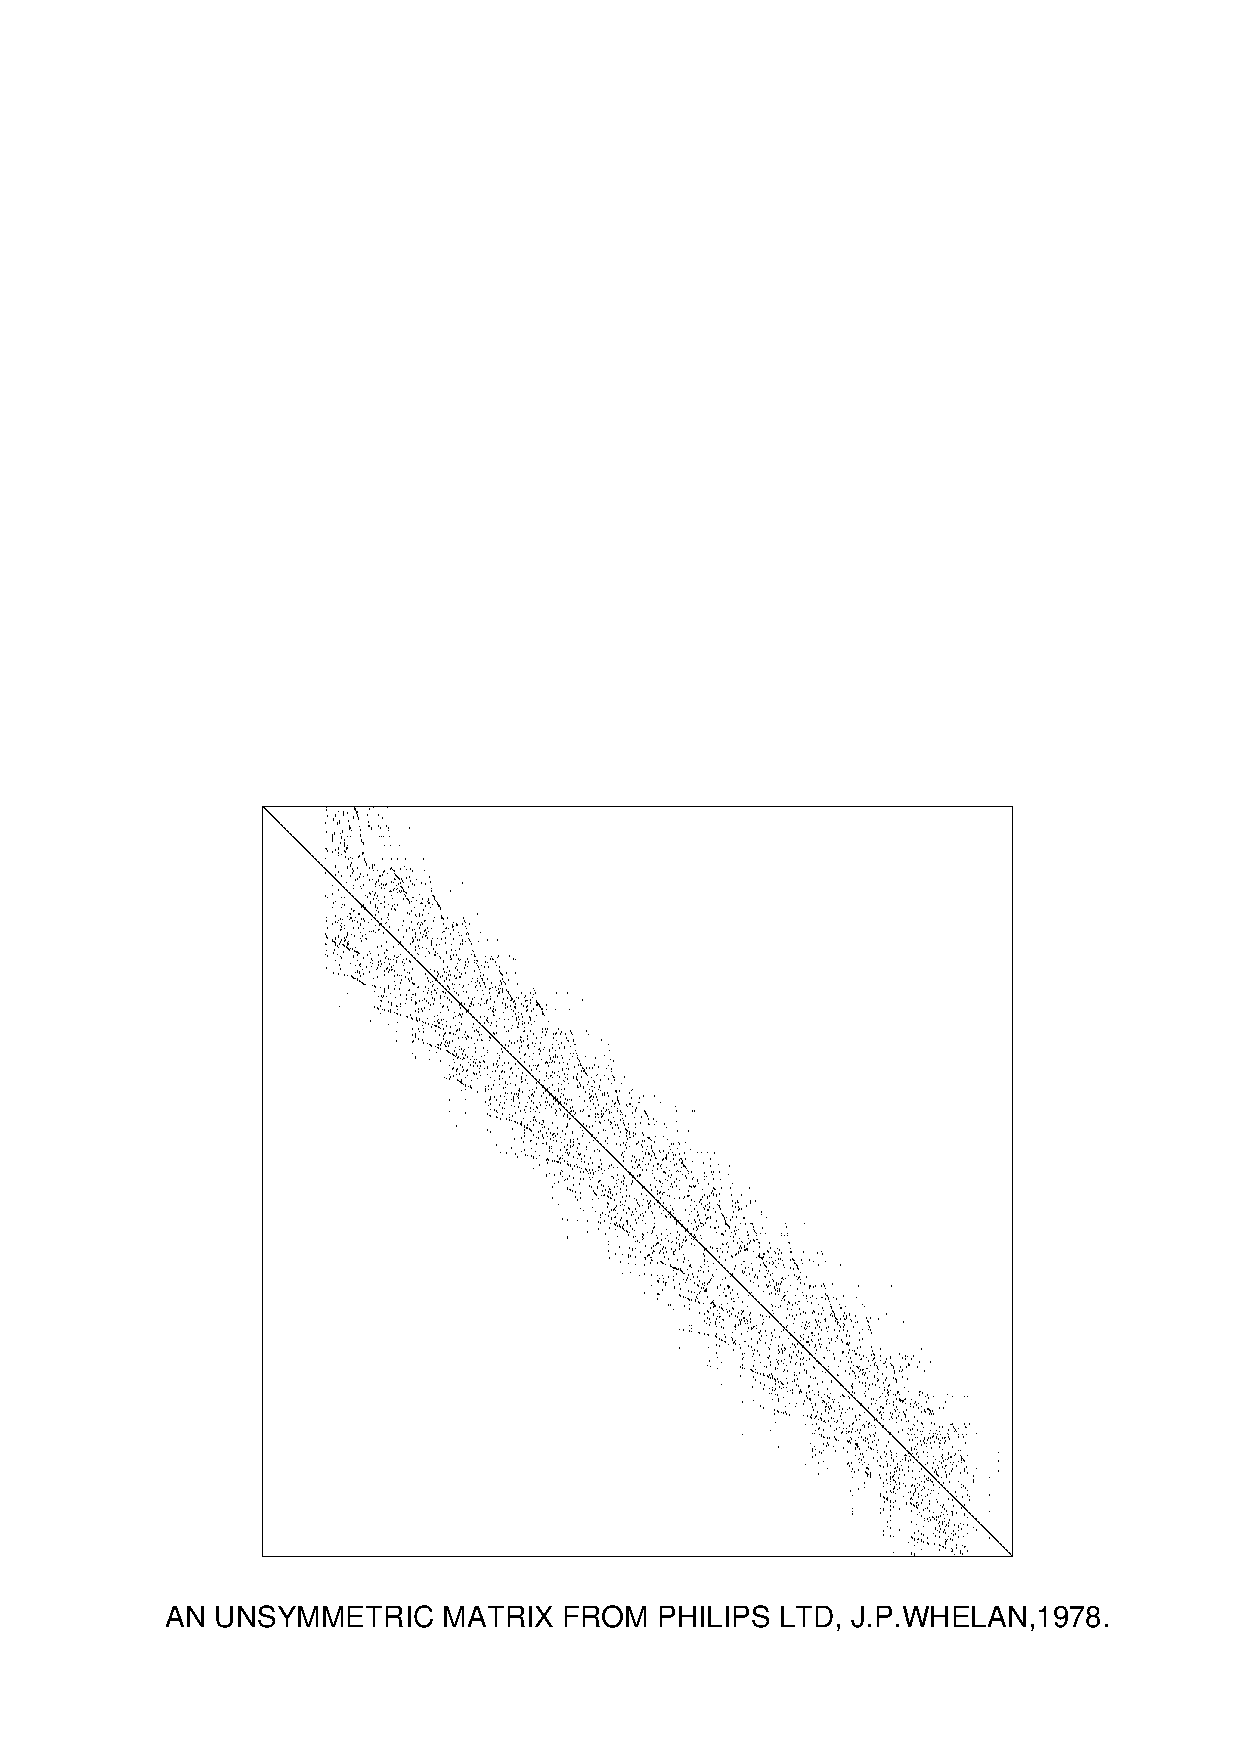
\includegraphics[width=5in]{jpwh}
%\vskip 5.5in
%\special{psfile=jpwh.ps vscale = 100 hscale = 100 hoffset = -85 voffset= -450}
%\special{psfile=jpwh.ps hoffset = -85}
\end{figure}

\section{Basic algebraic operations}
The usual algebraic operations involving two matrices,
such as $C= A+ B$, $C= A+\beta B$, $C= A B $, etc..,
are fairly common in sparse matrix computations.
These basic matrix operations
are included in the module called BLASSM.  In addition there is a
large number of basic operations, involving a sparse matrix
and a vector, such as matrix-vector products and
triangular system solutions that are very commonly used. Some of
these are included in the module MATVEC.
Sometimes it is desirable to compute the 
patterns of the matrices $A+B$ and $AB$, or in fact of any result 
of the basic algebraic  operations. This can be implemented by
way of job options which will determine whether to fill-in the real
values or not during the computation.  
We now briefly describe the contents of each of the 
two modules BLASSM and MATVEC. 

\subsection{The BLASSM module} 
Currently, the module BLASSM (Basic Linear Algebra Subroutines for
Sparse Matrices) contains the following nine subroutines:

\vskip 0.3in

\marg{ AMUB }\disp{ Performs the product of two matrices, i.e.,
computes $C = A B $, where $A$ and $B$ are both in CSR format.}

\marg{  APLB }\disp{ Performs the addition of two matrices, i.e.,
computes $C = A + B $, where $A$ and $B$ are both in CSR format.}

\marg{ APLSB }\disp{ Performs the operation $ C=A + \sigma B $, 
where $\sigma$ is a scalar, and $A, B$ are two matrices in 
CSR format. }

\marg{ APMBT }\disp{ Performs either the addition $C = A + B^T$ or the 
subtraction $C=A-B^T$.  }

\marg{ APLSBT }\disp{ Performs the operation $C = A + s B^T$. }

\marg{ DIAMUA }\disp{   Computes the product of diagonal 
matrix (from the left) by a sparse matrix, i.e.,
computes $C = D A$, where $D$ is a diagonal matrix and $A$
is a general sparse matrix stored in CSR format. }

\marg{ AMUDIA }\disp{ Computes the product of a sparse 
matrix by a diagonal matrix from the right, i.e., 
computes $C = A D $, where $D$ is a diagonal matrix and $A$
is a general sparse matrix stored in CSR format. }

\marg{ APLDIA }\disp{   Computes the sum of a sparse matrix and a 
diagonal matrix, $ C = A + D $.  }

\marg{ APLSCA }\disp{Performs an in-place
addition of a scalar to the diagonal entries of 
a sparse matrix, i.e., performs the operation
 $A := A + \sigma I$.} 

\vskip 0.3in 

Missing from this list are the routines {\bf AMUBT} which multiplies $A$ by 
the transpose of $B$, $C= AB^T$, and {\bf ATMUB } which multiplies the 
transpose of $A$ by $B$,	$C= A^T B $.

\vskip 0.3in

These are very difficult to implement and we found it better to 
perform it with two passes.
Operations of the form $ t A + s B $ have been
avoided as their occurrence does not warrant additional subroutines.
Several other operations similar to those defined for
vectors have not been included. For example the scaling
of a matrix  in sparse format is simply a scaling of its
real array $A$, which can be done with the usual BLAS1
scaling routine, on the array $A$. 


\subsection{The MATVEC module}
In its current status, this module contains matrix
by vector products and various sparse triangular 
solution methods. The contents are as follows.

\vskip 0.3in

\marg{ AMUX   }\disp{ Performs the product of a  matrix by a vector.
 Matrix stored in  Compressed Sparse Row (CSR) format.}

\marg{  ATMUX  }\disp{  Performs the product of the transpose of
a  matrix by a vector. Matrix $A$ stored in Compressed 
Sparse Row format. Can also be
viewed as the product of a matrix in the Compressed Sparse Column
format by a vector.} 

\marg{  AMUXE  }\disp{  Performs the product of a  matrix by a vector.
Matrix stored in  Ellpack/Itpack (ELL) format.}

\marg{ AMUXD  }\disp{  Performs the product of a  matrix by a vector.
Matrix stored in  Diagonal (DIA) format.}

\marg{ AMUXJ  }\disp{  Performs the product of a  matrix by a vector.
Matrix stored in  Jagged Diagonal (JAD) format.} 

\marg{ VBRMV }\disp{ Sparse matrix - full vector product in VBR format.} 

\marg{ LSOL } 
\disp{  Unit lower triangular system solution. Matrix stored in
Compressed Sparse Row (CSR) format. }

\marg{ LDSOL  }\disp{Lower triangular system solution. Matrix stored in
Modified Sparse Row (MSR) format. Diagonal elements inverted. }

\marg{ LSOLC  }\disp{ 
Unit lower triangular system solution. Matrix stored in
 Compressed Sparse Column (CSC) format.   }

\marg{ LDSOLC }\disp{  
Lower triangular system solution. Matrix stored in
Modified Sparse Column (MSC) format with diagonal elements inverted. }

\marg{ LDSOLL }\disp{ 
Unit lower triangular system solution with the level scheduling
approach.  Matrix 
stored in Modified Sparse Row format, with diagonal elements inverted.}

\marg{ USOL }\disp{  Unit upper triangular system solution. 
Matrix stored in Compressed Sparse Row (CSR) format. }

\marg{ UDSOL  }\disp{  Upper triangular system solution. 
Matrix stored in Modified Sparse Row (MSR) format. Diagonal 
elements inverted. }

\marg{ USOLC  }\disp{ 
Unit upper triangular system solution. Matrix stored in
Compressed Sparse Column (CSC) format.   } 

\marg{ UDSOLC }\disp{  
Upper triangular system solution. Matrix stored in
Modified Sparse Column (MSC) format with diagonal elements inverted. }

\vskip 0.3in
Most of the above routines are  short and rather straightforward.
A long test program  is provided to run all of the subroutines
on a large number of matrices that are dynamically generated
using the MATGEN module. 

\section{The basic statistics and information routines}
It is sometimes very  informative when analyzing
solution methods, to be able in a short amount of time to 
obtain some statistical information about a sparse matrix.
The purpose of the subroutine info1, is to print out such
information. The first question we had to address 
was to determine the type of information that
is inexpensive to obtain and yet practical and useful.
The simplest and most common statistics
are: total number of nonzero elements, average number of nonzero
elements per row (with standard deviation), band size.
Our preliminary package Info1 contains the above and a 
number of other features. For example it answers the following
questions: Is the matrix lower triangular, upper triangular?
does it have a symmetric structure? If not how close is it 
from having this property? Is it weakly row-diagonally dominant?
What percentage of the rows are weakly diagonally dominant?
Same questions for column diagonal dominance.
A sample output from  info1 is listed in 
Figure\ref{Fig1}. This print-out was  generated by typing 
\begin{center}
{\tt info1.ex < pores\_2}
\end{center}
%\[ {\rm info1.ex}  < {\rm pores\_2} \]
where {\tt pores\_2} is a file containing a matrix in H/B format.

If the Harwell-Boeing matrix is symmetric then Info1 takes this
information into account to obtain the correct information
instead of the information on  the lower triangular part only.
Moreover, in cases where only the pattern is provided (no real
values), then info1 will print a message to this effect and 
will then give information related only to the structure of 
the matrix. The output for an example of this type is shown in 
Figure~\ref{Fig2}. We should point out that the runs for these
two tests were basically instantaneous on a Sun-4 workstation.

Currently, this module contains the following subroutines:

\vskip 0.3in
 
\marg{ N\_IMP\_DIAG }\disp{ Computes the most important diagonals.}

\marg{ DIAG\_DOMI }\disp{ Computes the percentage of weakly diagonally 
dominant rows/columns.}

\marg{ BANDWIDTH }\disp{ Computes the lower, upper, maximum, and 
average bandwidths.}

\marg{ NONZ }\disp{ Computes maximum numbers of nonzero elements
per column/row, min numbers of nonzero elements per column/row,
and numbers of zero columns/rows.}

\marg{ FROBNORM }\disp{ Computes the Frobenius norm of A.}

\marg{ ANSYM }\disp{ Computes the Frobenius norm of the symmetric and
non-symmetric parts of A, computes the number of matching elements in symmetry 
and the relative symmetry match.
The routine ANSYM provides some information on the degree of symmetry of A.}

\marg{ DISTAIJ }\disp{ Computes the average distance of a(i,j) from diag and
standard deviation  for this average.}

\marg{ SKYLINE }\disp{ Computes the number of nonzeros in the skyline storage.}

\marg{ DISTDIAG }\disp{ Computes the numbers of elements in each diagonal.}

\marg{ BANDPART }\disp{ Computes the bandwidth of the banded matrix,
which contains 'nper' percent of the original matrix.}


\marg{ NONZ\_LUD }\disp{ Computes the number of nonzero elements in strict
lower part, strict upper part, and main diagonal.}

\marg{ AVNZ\_COL }\disp{ Computes average number of nonzero elements/column
and standard deviation for the average.}

\marg{ VBRINFO }\disp{ Prints information about matrices in variable block row 
format.}

% This has been updated to match the new code. -- June 3, 1994.
%* * * * * * * * * * * * * * * * * * * * * * * * * * * * * * * * * * * * * *
%* unsymmetric matrix from pores                                           *
%*                    Key = pores_2  , Type = rua                          *
%* * * * * * * * * * * * * * * * * * * * * * * * * * * * * * * * * * * * * *
%    *  Dimension N                                      =       1224  *
%    *  Number of nonzero elements                       =       9613  *
%    *  Average number of nonzero elements/Column        =     7.8538  *
%    *  Standard deviation for above average             =     5.4337  *
%    *  Nonzero elements in strict upper part            =       4384  *
%    *  Nonzero elements in strict lower part            =       4005  *
%    *  Nonzero elements in main diagonal                =       1224  *
%    *  Weight of longest column                         =         30  *
%    *  Weight of shortest column                        =          2  *
%    *  Weight of longest row                            =         30  *
%    *  Weight of shortest row                           =          2  *
%    *  Matching elements in symmetry                    =       6358  *
%    *  Relative Symmetry Match (symmetry=1)             =     0.6614  *
%    *  Average distance of a(i,j)  from diag.           =  0.615E+02  *
%    *  Standard deviation for above average             =  0.103E+03  *
%    *-----------------------------------------------------------------*
%    *  Frobenius norm of A                              =  0.150E+09  *
%    *  Frobenius norm of symmetric part                 =  0.100E+09  *
%    *  Frobenius norm of nonsymmetric part              =  0.951E+08  *
%    *  Maximum element in A                             =  0.378E+08  *
%    *  Percentage of weakly diagonally dominant rows    =  0.481E+00  *
%    *  Percentage of weakly diagonally dominant columns =  0.490E-02  *
%    *-----------------------------------------------------------------*
%    *  Lower bandwidth  (max: i-j, a(i,j) .ne. 0)       =        470  *
%    *  Upper bandwidth  (max: j-i, a(i,j) .ne. 0)       =        471  *
%    *  Maximum Bandwidth                                =        736  *
%    *  Average Bandwidth                                =  0.190E+03  *
%    *  Number of nonzeros in skyline storage            =     340385  *
%    *  90% of matrix is in the band of width            =        527  *
%    *  80% of matrix is in the band of width            =        145  *
%    *  The total number of nonvoid diagonals is         =        367  *
%    *  The 10 most important diagonals are (offsets)    :             *
%    *     0     1    -1    -2     2    -3   -32  -264   264    32     *
%    *  The accumulated percentages they represent are   :             *   
%    *  12.7  24.6  31.7  37.9  43.6  49.0  52.4  55.7  58.6  61.4     *
%    *-----------------------------------------------------------------*
%    *  The matrix does not have a block structure                     *
%    *-----------------------------------------------------------------*
\begin{figure}
\begin{verbatim}
* * * * * * * * * * * * * * * * * * * * * * * * * * * * * * * * * * * * * *
* UNSYMMETRIC MATRIX FROM PORES                                           *
*                    Key = PORES 2  , Type = RUA                          *
* * * * * * * * * * * * * * * * * * * * * * * * * * * * * * * * * * * * * *
    *  Dimension N                                      =       1224  *
    *  Number of nonzero elements                       =       9613  *
    *  Average number of nonzero elements/Column        =     7.8538  *
    *  Standard deviation for above average             =     5.4337  *
    *  Nonzero elements in strict lower part            =       4384  *
    *  Nonzero elements in strict upper part            =       4005  *
    *  Nonzero elements in main diagonal                =       1224  *
    *  Weight of longest column                         =         30  *
    *  Weight of shortest column                        =          2  *
    *  Weight of longest row                            =         16  *
    *  Weight of shortest row                           =          5  *
    *  Matching elements in symmetry                    =       6358  *
    *  Relative Symmetry Match (symmetry=1)             =     0.6614  *
    *  Average distance of a(i,j)  from diag.           =  0.615E+02  *
    *  Standard deviation for above average             =  0.103E+03  *
    *-----------------------------------------------------------------*
    *  Frobenius norm of A                              =  0.150E+09  *
    *  Frobenius norm of symmetric part                 =  0.103E+09  *
    *  Frobenius norm of nonsymmetric part              =  0.980E+08  *
    *  Maximum element in A                             =  0.378E+08  *
    *  Percentage of weakly diagonally dominant rows    =  0.490E-02  *
    *  Percentage of weakly diagonally dominant columns =  0.481E+00  *
    *-----------------------------------------------------------------*
    *  Lower bandwidth  (max: i-j, a(i,j) .ne. 0)       =        470  *
    *  Upper bandwidth  (max: j-i, a(i,j) .ne. 0)       =        471  *
    *  Maximum Bandwidth                                =        736  *
    *  Average Bandwidth                                =  0.190E+03  *
    *  Number of nonzeros in skyline storage            =     342833  *
    *  90% of matrix is in the band of width            =        527  *
    *  80% of matrix is in the band of width            =        145  *
    *  The total number of nonvoid diagonals is         =        367  *
    *  The 10 most important diagonals are (offsets)    :             *
    *     0    -1     1     2    -2     3    32   264  -264   -32     *
    *  The accumulated percentages they represent are   :             *
    *  12.7  24.6  31.7  37.9  43.6  49.0  52.4  55.7  58.6  61.4     *
    *-----------------------------------------------------------------*
    *  The matrix does not have a block structure                     *
    *-----------------------------------------------------------------*
\end{verbatim}
\caption{Sample output from Info1.ex \label{Fig1} } 
\end{figure}


%* * * * * * * * * * * * * * * * * * * * * * * * * * * * * * * * * * * * * *
%* SYMMETRIC PATTERN FROM CANNES,LUCIEN MARRO,JUNE 1981.                   *
%*                    Key = CAN 1072 , Type = PSA                          *
%* No values provided - Information on pattern only                        *
%* * * * * * * * * * * * * * * * * * * * * * * * * * * * * * * * * * * * * *
%    *  Dimension N                                      =       1072  *
%    *  Number of nonzero elements                       =       6758  *
%    *  Average number of nonzero elements/Column        =    11.6082  *
%    *  Standard deviation for above average             =     5.6474  *
%    *  Nonzero elements in strict upper part            =       5686  *
%    *  Nonzero elements in strict lower part            =       5686  *
%    *  Nonzero elements in main diagonal                =       1072  *
%    *  Weight of longest column                         =         35  *
%    *  Weight of shortest column                        =          6  *
%    *  Matching elements in symmetry                    =       6758  *
%    *  Relative Symmetry Match (symmetry=1)             =     1.0000  *
%    *  Average distance of a(i,j)  from diag.           =  0.110E+03  *
%    *  Standard deviation for above average             =  0.174E+03  *
%    *-----------------------------------------------------------------*
%    *  Lower bandwidth  (max: i-j, a(i,j) .ne. 0)       =       1048  *
%    *  Upper bandwidth  (max: j-i, a(i,j) .ne. 0)       =       1048  *
%    *  Maximum Bandwidth                                =       1055  *
%    *  Average Bandwidth                                =  0.376E+03  *
%    *  Number of nonzeros in skyline storage            =     277248  *
%    *  90% of matrix is in the band of width            =        639  *
%    *  80% of matrix is in the band of width            =        343  *
%    *  The total number of nonvoid diagonals is         =        627  *
%    *  The  5 most important diagonals are (offsets)    :             *
%    *     0    -1    -2    -3    -4                                   *
%    *  The accumulated percentages they represent are   :             *
%    *  15.9  24.7  29.7  33.9  36.3                                   *
%    *-----------------------------------------------------------------*
%    *  The matrix does not have a block structure                     *
%    *-----------------------------------------------------------------*
\begin{figure}
\begin{verbatim}
* * * * * * * * * * * * * * * * * * * * * * * * * * * * * * * * * * * * * *
* SYMMETRIC PATTERN FROM CANNES,LUCIEN MARRO,JUNE 1981.                   *
*                    Key = CAN 1072 , Type = PSA                          *
* No values provided - Information on pattern only                        *
* * * * * * * * * * * * * * * * * * * * * * * * * * * * * * * * * * * * * *
    *  Dimension N                                      =       1072  *
    *  Number of nonzero elements                       =       6758  *
    *  Average number of nonzero elements/Column        =     6.3041  *
    *  Standard deviation for above average             =     6.2777  *
    *  Nonzero elements in strict lower part            =       5686  *
    *  Nonzero elements in strict upper part            =       5686  *
    *  Nonzero elements in main diagonal                =       1072  *
    *  Weight of longest column                         =         39  *
    *  Weight of shortest column                        =          4  *
    *  Matching elements in symmetry                    =       6758  *
    *  Relative Symmetry Match (symmetry=1)             =     1.0000  *
    *  Average distance of a(i,j)  from diag.           =  0.110E+03  *
    *  Standard deviation for above average             =  0.174E+03  *
    *-----------------------------------------------------------------*
    *  Lower bandwidth  (max: i-j, a(i,j) .ne. 0)       =          0  *
    *  Upper bandwidth  (max: j-i, a(i,j) .ne. 0)       =       1048  *
    *  Maximum Bandwidth                                =       1049  *
    *  Average Bandwidth                                =  0.117E+03  *
    *  Number of nonzeros in skyline storage            =     278320  *
    *  90% of matrix is in the band of width            =        639  *
    *  80% of matrix is in the band of width            =        343  *
    *  The total number of nonvoid diagonals is         =        627  *
    *  The  5 most important diagonals are (offsets)    :             *
    *     0     1     2     3     4                                   *
    *  The accumulated percentages they represent are   :             *
    *  15.9  24.7  29.7  33.9  36.3                                   *
    *-----------------------------------------------------------------*
    *  The matrix does not have a block structure                     *
    *-----------------------------------------------------------------*
\end{verbatim}
\caption{Sample output from Info1.ex for matrix with pattern only \label{Fig2}}
\end{figure}

%% \vfill 

\section{Matrix generation routines}
One of the difficulties encountered when testing and comparing
numerical methods, is that it is sometimes difficult to 
guarantee that the matrices compared are indeed identical.
Even though a paper may give full details on the test
problems considered, programming errors or differences in coding
may lead to the incorrect matrices and the incorrect conclusions.
This has often happened in the past and is likely to be avoided  if 
the matrices were generated with exactly the same code. 
The module MATGEN of
SPARSKIT includes several matrix generation routines.

\subsection{Finite Difference Matrices}

\begin{enumerate}
\item Scalar 5-point and 7-point matrices arising 
from discretization of the elliptic type equation:
\begin{equation}
L u = {\del \over \del x} ( a   {\del \over \del x } u ) 
+ {\del \over \del y } ( b   {\del \over \del y }  u) 
+ {\del \over \del z } ( c   {\del \over \del z } u ) 
+ {\del \over \del x } ( d   u ) + {\del \over \del y }  (e   u) 
+ {\del \over \del z } ( f   u ) + g   u  = h u
\label{5-7pt}
\end{equation} 
on rectangular regions with general mixed type boundary conditions of
the following form
\[ \alpha {\del u \over \del n} + \beta u = \gamma \]
The user provides the functions $a, b, c, ...,h$, $\beta, \gamma$ and
$\alpha$ is a constant on each boundary surface. The resulting 
matrix is in general sparse format, possibly printed in a file
in the H/B format. 

There is a switch in the subroutine which makes it possible to choose
between a strict centered difference type of discretization, or an
upwind scheme for the first order derivatives.

\item
Block 5-point and 7-point matrices arising 
from discretization of the elliptic type equation \nref{5-7pt}
in which $u$ is now a vector of $nfree$ components, and
$a,b,c, ..., g$ are $nfree \times  nfree $ matrices provided by the
user.

\end{enumerate}

\subsection{Finite Element Matrices}

Finite element matrices created from the convection-diffusion type problem 
\begin{equation} - \nabla . ({ K \nabla u }) + {C \nabla u} = f \label{kikuchi} 
\end{equation}
on a domain $D$ with Dirichlet boundary conditions.  A coarse initial domain
is described by the user and the code does an arbitrary user-specified number
of refinements of the grid and assembles the matrix, in CSR format.
Linear triangular elements are used.  If only the matrix is desired the heat
source $f$ can be zero. Arbitrary grids can be input, but the user may 
also take advantage of nine initial grids
supplied by the package for simple test problems. 

Two examples of meshes and the corresponding assemble matrices are shown
in the following two pairs of figures: the first pair of figures are the mesh 
and assembled matrix with mesh number 8 and refinement 1; the second pair of
figures are the mesh and assembled matrix with mesh number 9 and refinement 1.

\begin{figure}[b]
\begin{minipage}[h]{6.5cm}
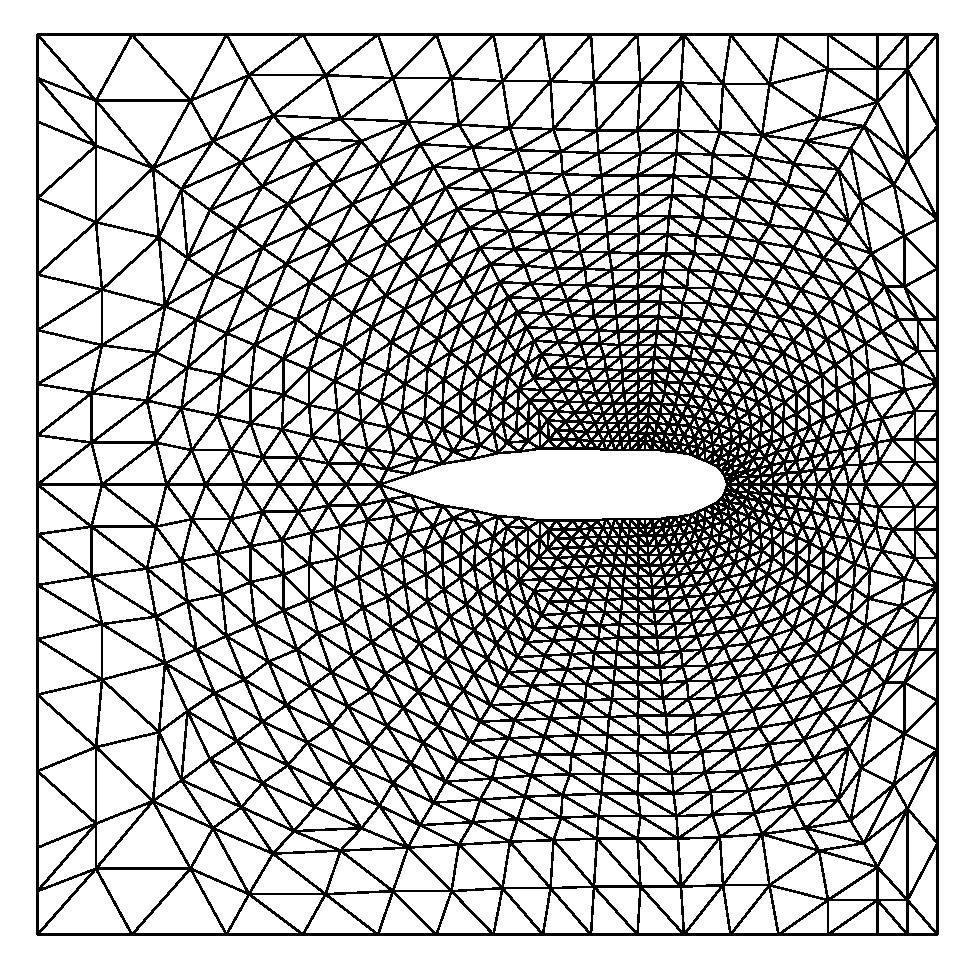
\includegraphics[height=5cm]{msh8} 
\end{minipage}
\hfill
\begin{minipage}[h]{6.5cm}
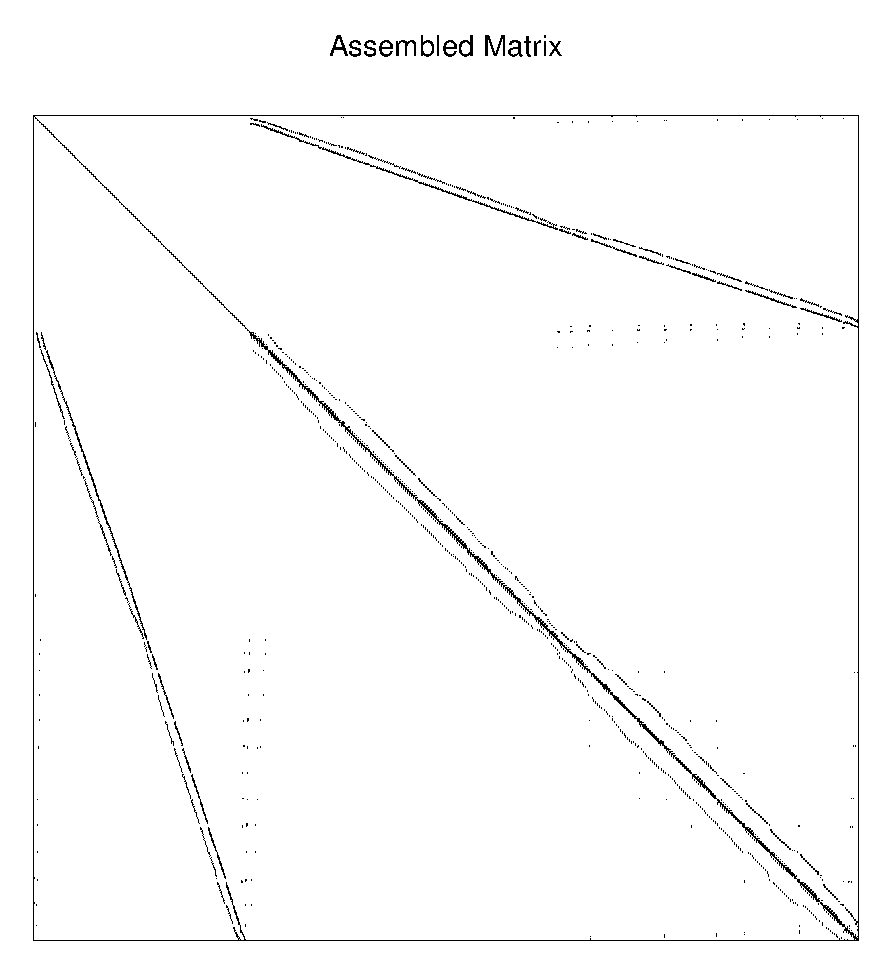
\includegraphics[height=5cm]{mat8}
\end{minipage}
\hfill
\end{figure}

\newpage

\begin{figure}
\begin{minipage}[h]{6.5cm}
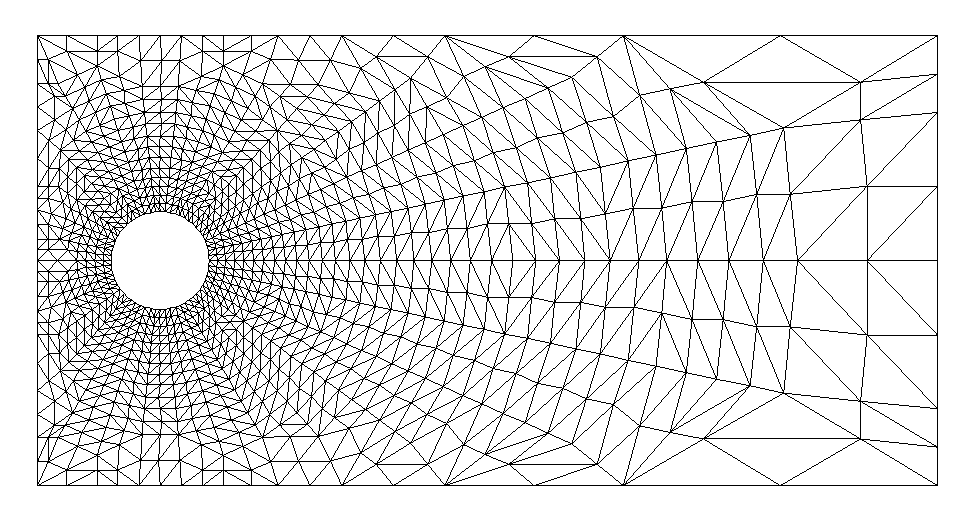
\includegraphics[width=8cm]{msh9} 
\end{minipage}
\hfill
\begin{minipage}[h]{6.5cm}
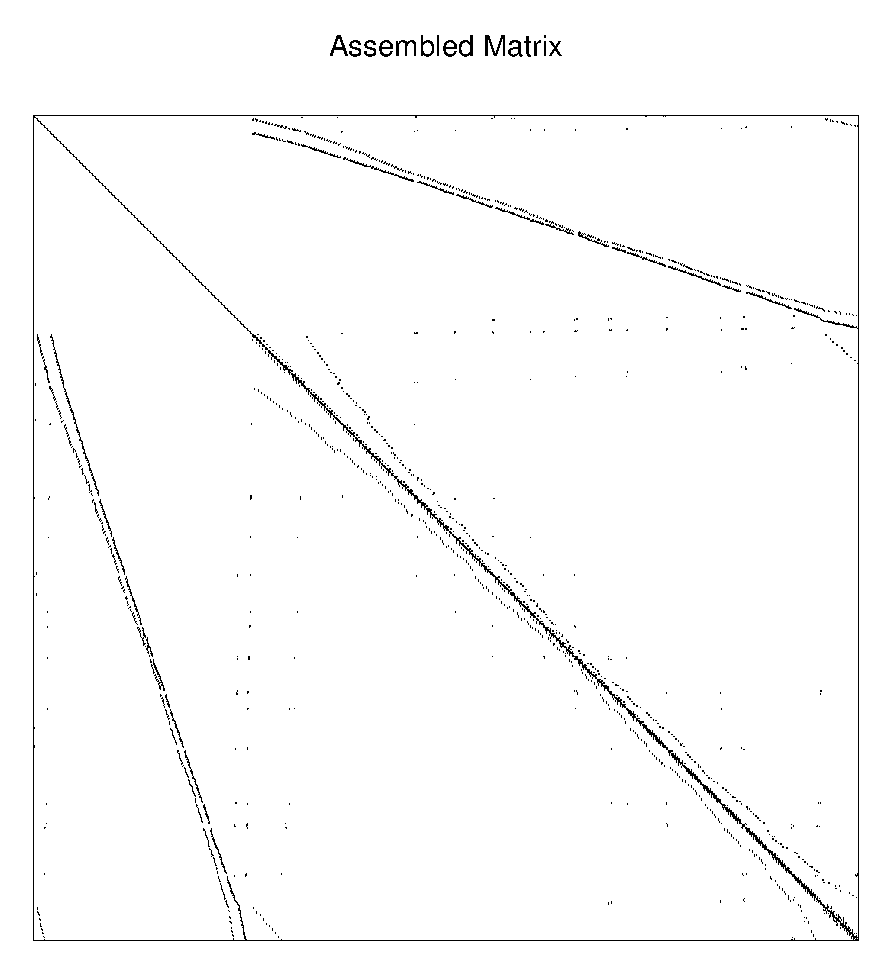
\includegraphics[height=7cm]{mat9}
\end{minipage}
\hfill
\end{figure}

\vskip 2.5in
\subsection{Markov Chains}

Markov chain matrices arising from a random walk on a
triangular grid. This is mainly useful for testing nonsymmetric 
eigenvalue codes. It has been suggested by G.W. Stewart in one of his
papers \cite{Stewart-SRRIT} and was used by Y. Saad in a few
subsequent papers as a test problem for nonsymmetric eigenvalue methods,
see,  e.g., \cite{Saad-cheb}. 

\subsection{Other Matrices}

Currently we have only one additional set of matrices. These are
the test matrices
\footnote{These subroutines have been contributed 
to the author by E. Rothman from Cornell University.} from 
Zlatev et. al. \cite{Zlatev-tests} and Osterby and Zlatev
\cite{OsterbyZlatev-book}. The first two matrix generators
described in the above references 
are referred to as $D(n,c) $ and $E(n,c)$ respectively.
A more elaborate class where more than two parameters can be varied,
is referred to as the class $F(m,n,c,r,\alpha) $ in
\cite{OsterbyZlatev-book,Zlatev-tests}. The three subroutines to generate
these matrices are called MATRF2 (for the class $F(m,n,c,r,\alpha)$ ),
DCN (for the class $D(c,n)$) and ECN (for the class $E(c,n) $).
These codes can generate rectangular as well as square 
matrices and allow a good flexibility in making the matrices 
more or less dense and more or less well conditioned.

\section{The ORDERING Routines}
The following subroutines are available in the directory ORDERINGS.

\vskip 0.3in

\marg{ levset.f }\disp{Reordering based on level sets, including
Cuthill-McKee implemented with breadth first search.}

\marg{ color.f }\disp{Reordering based on coloring, including a greedy 
algorithm for multicolor ordering.}

\marg{ ccn.f }\disp{Reordering routines based on strongly connected
components.  Contributed by Laura C. Dutto (CERCA and Concordia
University.}


\section{The ITSOL routines}

\marg{ILUT}\disp{This file contains a preconditioned GMRES algorithm 
  with four preconditioners:}
\marg{pgmres}\disp{Preconditioned GMRES solver.  This solver may be used
  with all four of the precondioners below.  Supports right preconditioning 
  only.}
\marg{ilut}\disp{ A robust preconditioner called ILUT 
 which uses a dual thresholding strategy for dropping elements.
 Arbitrary accuracy is allowed in ILUT.}
\marg{ilutp}\disp{ ILUT with partial pivoting}
\marg{ilu0}\disp{ simple ILU(0) preconditioner}
\marg{milu0}\disp{ MILU(0) preconditioner}

\marg{ITERS}\disp{This file currently has several basic iterative linear 
 system solvers which use reverse communication. They are:}
\marg{cg}\disp{Conjugate Gradient Method}
\marg{cgnr}\disp{Conjugate Gradient Method\-- for Normal Residual equation}
\marg{bcg}\disp{Bi\-Conjugate Gradient Method}
\marg{bcgstab}\disp{BCG stablized}
\marg{tfqmr}\disp{Transpose\-Free Quasi\-Minimum Residual method}
\marg{gmres}\disp{Generalized Minimum Residual method}
\marg{fgmres}\disp{Flexible version of Generalized Minimum Residual method}
\marg{dqgmres}\disp{Direct versions of Quasi Generalized Minimum Residual
                       method}
\marg{dbcg}\disp{BCG with partial pivoting}


\section{The UNSUPP directory}
In addition to the basic tools described in the previous 
sections, SPARSKIT includes a directory 
called UNSUPP includes software that is not necessarily 
portable or that does not fit in all previous modules.
For example software for viewing matrix patterns on 
some particular workstation
may be found here. Another example is 
routines related to matrix exponentials.
%all the different
%reordering schemes, such as minimum degree ordering, or
%nested dissection etc.. 
Many of these are available from
NETLIB but others may be contributed by researchers for
comparison purposes.

%The  two basic programs for viewing matrix patterns on
%a sun screen will eventually be replaced by 
%programs for the X-windows environment which is fast becoming
%a standard. 

%There are three subdirecitories in this directory.
%\subsection{Blas1}
%The following items are available in Blas1.
%
%\vskip 0.3in
%
%\marg{dcopy} \disp{copies a vector, x, to a vector, y.}
%\marg{ddot}  \disp{dot product of two vectors.}
%\marg{csscal}\disp{scales a complex vector by a real constant.}
%\marg{cswap} \disp{interchanges two vectors.}
%\marg{csrot} \disp{applies a plane rotation.}
%\marg{cscal} \disp{scales a vector by a constant.}
%\marg{ccopy} \disp{copies a vector, x, to a vector, y.}
%\marg{drotg} \disp{construct givens plane rotation.}
%\marg{drot}  \disp{applies a plane rotation.}
%\marg{dswap} \disp{interchanges two vectors.}
%\marg{dscal} \disp{scales a vector by a constant.}
%\marg{daxpy} \disp{constant times a vector plus a vector.}


\subsection{Plots}
The following items are available in PLOTS. 

\vskip 0.3in

%\marg{ PLTMTPS}\disp{ a translation of the pltmt subroutine 
%  in INOUT/inout.f
%  to produce a post-script file rather than a pic file. 
%  Does not yet offer the same functionality as pltmt. } 
%
%\marg{ HB2PIC}\disp{ reads a Harwell-Boeing 
%  matrix and creates a picture file for pattern.}
%
%\marg{ HB2PS}\disp{translates a Harwell-Boeing file into a 
%Post-Script file.}

\marg{ PSGRD}\disp{ contains subroutine "psgrid" which plots 
  a symmetric graph.}

%\marg{ RUNPS}\disp{ contains subroutine "rpltps" which reads 
%  a Harwell-Boeing file from standard input and creates a  
%  Post-Script file for it}

\marg{ TEXPLT1}\disp{ contains subroutine "texplt" allows 
  several matrices in the same picture by calling texplt several 
  times and exploiting job and different shifts.}

\marg{ TEXGRID1}\disp{ contains subroutine "texgrd" which  
  generates tex commands for plotting a symmetric graph associated
  with a mesh. Allows several grids in the same picture by 
  calling texgrd several times and exploiting job and different 
  shifts.}  


\subsection{Matrix Exponentials}
Two subroutines are available in this directory.
\vskip 0.3in
\marg{ EXPPRO}\disp{ A subroutine for computing the product of a matrix 
  exponential times a vector, i.e. $w = exp(t\ A)\ v$.}
\marg{ PHIPRO}\disp{ computes $w = \phi(A\ t)\ v$,
  where $\phi(x) = (1-exp(x))/x$; Also can solve the 
  system of ODE's $ y'= A y + b$.}

\section{Distribution}
The SPARSKIT package 
follows the Linpack-Eispack approach in that it  aims at providing
efficient and well tested subroutines written in portable FORTRAN.
Similarly to the Linpack and Eispack packages, the goal is to
make available a common base of useful codes for a specific 
area of computation, in this case sparse linear algebra.
The package is in the public domain and will be made 
accessible through the internet.

See Figure \ref{organization} for an illustration of the organization
of SPARSKIT.  Read the README file in the main directory for more
information.

%Currently, the package is organized in six distinct subdirectories,
%each containing one or more modules. The six directories 
%and the modules they contain are the following:
%INOUT (inout.f), FORMATS (formats.f, unary.f), BLASSM (blassm.f,
%matvec.f), MATGEN (genmat.f, zlatev.f), INFO (dinfo1.f), 
%UNSUPP (various routines).   Test programs with unix makefiles
%are provided in each
%subdirectory to test a large number of the subroutines.
%Each directory contains a README file listing contents,
%and giving additional information. 

For information concerning distribution contact the author at
%%saad@riacs.edu.
saad@cs.umn.edu.

\section{Conclusion and Future Plans}
It is hoped that SPARSKIT will be useful in many 
ways to researchers in different areas of scientific computing.
In this version of SPARSKIT, there are few sparse
problem solvers, such as direct solution methods, or 
eigenvalue solvers. Some of these are available from different
sources and we felt that it was not appropriate to provide
additional ones. The original 
motivation for SPARSKIT is  that there is 
a gap to fill in the manipulation and basic computations
with sparse matrices. Once this gap is filled with some
satisfaction, then additional functionality may be added.

We briefly mentioned in the introduction the possibility of using 
SPARSKIT to develop an interactive package.
Large matrices of dimension tens of of thousands can 
easily be manipulated with the current supercomputers, 
in real time. One of the difficulties
with such an interactive package is that we do not yet
have reliable routines for computing eigenvalues/eigenvectors of
large sparse matrices. The state of the art in solving linear 
systems is in a much better situation. However, one must not 
contemplate performing the same type of computations as with 
small dense matrices. As an example,
getting all the eigenvalues of a sparse matrix is not likely
to be too useful when the matrix is very large.

Beyond interactive software for sparse linear algebra, one can
envision the integration of SPARSKIT in a larger package 
devoted to solving certain types of Partial Differential Equations, 
possibly interactively. 

\vskip 1.3in
\noindent
{\bf Acknowledgements.} The idea of creating a tool package for
sparse matrices germinated while the author was at the Center for 
Supercomputing Research and Development of the University of Illinois
(1986-1987) and part of this work was performed there. 
Initially the author has benefited from helpful comments from Iain Duff
(then visiting CSRD) and a number of colleagues at CSRD.  
Billy Stewart and his students at NCSU used a preliminary version of 
SPARSKIT in a class project and made some
valuable comments. Ernie Rothman (Cornell) and
Laura Dutto (Montreal) contributed some software.
The author has also benefited from helpful discussions
from a number of other colleagues, including 
Mike Heroux, Giuseppe Radicatti, Ahmed Sameh, Horst Simon, 
Phuong Vu, and Harry Wijshoff.  Students who contributed to
version 2 of SPARSKIT include Kesheng Wu, Edmond Chow, and Dongli Su.

\newpage
\begin{thebibliography}{10}

\bibitem{Anderson-Saad}
E.~C. Anderson and Y.~Saad.
\newblock Solving sparse triangular systems on parallel computers.
\newblock Technical Report 794, University of Illinois, CSRD, Urbana, IL, 1988.

\bibitem{Duff-survey}
I.~S. Duff.
\newblock A survey of sparse matrix research.
\newblock In {\em Proceedings of the IEEE, 65}, pages 500--535, New York, 1977.
  Prentice Hall.

\bibitem{Duff-book}
I.~S. Duff, {A. M. Erisman}, and {J. K. Reid}.
\newblock {\em Direct Methods for Sparse Matrices}.
\newblock Clarendon Press, Oxford, 1986.

\bibitem{Duff-HB}
I.~S. Duff, R.~G. Grimes, and J.~G. Lewis.
\newblock Sparse matrix test problems.
\newblock {\em ACM trans. Math. Soft.}, 15:1--14, 1989.

\bibitem{Oppe-NSPCG}
T.~C. Oppe~Wayne Joubert and D.~R. Kincaid.
\newblock Nspcg user's guide. a package for solving large linear systems by
  various iterative methods.
\newblock Technical report, The University of Texas at Austin, 1988.

\bibitem{Oppe-Kincaid}
T.~C. Oppe and D.~R. Kincaid.
\newblock The performance of {ITPACK} on vector computers for solving large
  sparse linear systems arising in sample oil reservoir simulation problems.
\newblock {\em Communications in applied numerical methods}, 2:1--7, 1986.

\bibitem{OsterbyZlatev-book}
O.~Osterby and Z.~Zlatev.
\newblock {\em Direct methods for sparse matrices}.
\newblock Springer Verlag, New York, 1983.

\bibitem{Saad-cheb}
Y.~Saad.
\newblock {Chebyshev} acceleration techniques for solving nonsymmetric
  eigenvalue problems.
\newblock {\em Mathematics of Computation}, 42:567--588, 1984.

\bibitem{Saad-Boeing}
Y.~Saad.
\newblock {Krylov} subspace methods on supercomputers.
\newblock {\em SIAM J. Scient. Stat. Comput.}, 10:1200--1232, 1989.

\bibitem{Stewart-SRRIT}
G.W. Stewart.
\newblock {SRRIT} - a FORTRAN subroutine to calculate the dominant invariant
  subspaces of a real matrix.
\newblock Technical Report TR-514, University of Maryland, College Park, MD,
  1978.

\bibitem{Young-Oppe-al}
D.~M. Young, T.C. Oppe, D.~R. Kincaid, and L.~J. Hayes.
\newblock On the use of vector computers for solving large sparse linear
  systems.
\newblock Technical Report CNA-199, Center for Numerical Analysis, University
  of Texas at Austin, Austin, Texas, 1985.

\bibitem{Zlatev-tests}
Z.~Zlatev, K.~Schaumburg, and J.~Wasniewski.
\newblock A testing scheme for subroutines solving large linear problems.
\newblock {\em Computers and Chemistry}, 5:91--100, 1981.

\end{thebibliography}
%%

\newpage

\appendix
\centerline{\bf APPENDIX: QUICK REFERENCE}
\vskip 0.3in

For convenience we list in this 
appendix the most important subroutines in the various
modules of SPARSKIT. More detailed information can be found either
in the body of the paper or in the documentation of the package.

\vskip 0.3in
\centerline{\bf FORMATS Module} 

\begin{itemize} 

\item CSRDNS  : converts a row-stored sparse matrix into the dense format. 
\item DNSCSR  : converts a dense matrix to a sparse storage format.        
\item COOCSR  : converts coordinate to  to csr format                      
\item COICSR  : in-place conversion of coordinate to csr format            
\item CSRCOO  : converts compressed sparse row to coordinate format.
\item CSRSSR  : converts compressed sparse row to symmetric sparse row format.
\item SSRCSR  : converts symmetric sparse row to compressed sparse row format.
\item CSRELL  : converts compressed sparse row to Ellpack format           
\item ELLCSR  : converts Ellpack format to compressed sparse row format.
\item CSRMSR  : converts compressed sparse row format to modified sparse   
           row format.
\item MSRCSR  : converts modified sparse row format to compressed sparse   
           row format.
\item CSRCSC  : converts compressed sparse row format to compressed sparse 
           column format (transposition).
\item CSRLNK  : converts compressed sparse row to linked list format.
\item LNKCSR  : converts linked list format to compressed sparse row fmt.
\item CSRDIA  : converts the compressed sparse row format into the diagonal    
           format.                                                    
\item DIACSR  : converts the diagonal format into the compressed sparse row    
           format.                                                    
\item BSRCSR  : converts the block-row sparse format into the compressed       
           sparse row format.                                         
\item CSRBSR  : converts the compressed sparse row format into the block-row   
           sparse format.                                             
\item CSRBND  : converts the compressed sparse row format into the  banded   
           format (Linpack style).                                    
\item BNDCSR  : converts the banded format (Linpack style) into the compressed 
           sparse row storage.                                        
\item CSRSSK  : converts the compressed sparse row format to the symmetric
           skyline format                                           
\item SSKSSR  : converts symmetric skyline format to symmetric
sparse row           format.                             
\item CSRJAD  : converts the csr format into the jagged diagonal format.
\item JADCSR  : converts the jagged-diagonal format into the csr format.
\item CSRUSS  : converts the csr format to unsymmetric sparse skyline format.
\item USSCSR  : converts unsymmetric sparse skyline format to the csr format.
\item CSRSSS  : converts the csr format to symmetric sparse skyline format.
\item SSSCSR  : converts symmetric sparse skyline format to the csr format.
\item CSRVBR  : converts compressed sparse row into variable block row format.
\item VBRCSR  : converts the variable block row format into the
\item COOELL  : converts the coordinate format into the Ellpack/Itpack format.
compressed sparse row format.
\end{itemize}

\vskip 0.3in
\centerline{\bf UNARY Module}

\begin{itemize} 

\item SUBMAT : extracts a submatrix from a sparse matrix.                  
\item FILTER : filters elements from a matrix according to their magnitude.
\item FILTERM: Same as above, but for the MSR format.
\item TRANSP : in-place transposition routine (see also CSRCSC in formats) 
\item GETELM : returns $a(i,j)$ for any $(i,j)$	 from a CSR-stored matrix.
\item COPMAT : copies a matrix into another matrix (both stored csr).
\item MSRCOP : copies a matrix in MSR format into a matrix in MSR format.
\item GETELM : returns a(i,j) for any (i,j) from a CSR-stored matrix.
\item GETDIA : extracts a specified diagonal from a matrix.                
\item GETL   : extracts lower triangular part.
\item GETU   : extracts upper triangular part.                             
\item LEVELS : gets the level scheduling structure for lower triangular    
 matrices.                                                   
\item AMASK  : extracts  $C = A \odot  M $
\item RPERM  : permutes the rows of a matrix ($B = P A$)                     
\item CPERM  : permutes the columns of a matrix ($B = A Q$)                  
\item DPERM  : permutes a matrix ($B = P A Q$) given two permutations P, Q   
\item DPERM2 : general submatrix permutation/extraction routine.
\item DMPERM : symmetric permutation of row and column (B=PAP') in MSR fmt.
\item DVPERM : permutes a vector (in-place).                                
\item IVPERM : permutes an integer vector (in-place).
\item RETMX  : returns the max absolute value in each row of the matrix.
\item DIAPOS : returns the positions of the diagonal elements in A.
\item EXTBDG : extracts the main diagonal blocks of a matrix.   
\item GETBWD : returns the bandwidth information on a matrix.              
\item BLKFND : finds the block-size of a matrix.        
\item BLKCHK : checks whether a given integer is the block size of $A$.
\item INFDIA : obtains information on the diagonals of $A$.    
\item AMUBDG : computes the number of nonzero elements in each 
	row of $A*B$.
\item APLBDG : computes the number of nonzero elements in each 
	row of $ A+B$. 
\item RNRMS  : computes the norms of the rows of $A$.                
\item CNRMS  : computes the norms of the columns of $A$.                      
\item ROSCAL : scales the rows of a matrix by their norms.                 
\item COSCAL : scales the columns of a matrix by their norms.              
\item ADDBLK : adds a matrix B into a block of A. 
\item GET1UP : collects the first elements of each row of the upper
               triangular portion of the matrix.
\item XTROWS : extracts given rows from a matrix in CSR format.

\end{itemize}

\vskip 0.3in
\centerline{\bf INOUT Module} 

\begin{itemize} 

\item  READMT : reads matrices in the boeing/Harwell format.               
\item  PRTMT  : prints matrices in the boeing/Harwell format.   
\item  DUMP   : prints rows of a matrix,  in a readable format.
\item  PLTMT  : produces a 'pic' file for plotting a sparse matrix.
\item PSPLTM  : Generates a post-script plot of the non-zero 
pattern of A.
\item SMMS    : Write the matrix in a format used in SMMS package.
\item READSM  : Reads matrices in coordinate format (as in SMMS 
package).
\item READSK  : Reads matrices in CSR format (simplified H/B formate).
\item SKIT    : Writes matrices to a file, format same as above.
\item PRTUNF  : Writes matrices (in CSR format) unformatted.
\item READUNF : Reads unformatted data of matrices (in CSR format).
\end{itemize}

\vskip 0.3in
\centerline{\bf INFO Module}

\begin{itemize} 
\item INFOFUN :  routines for statistics on a sparse matrix.
\end{itemize}

\vskip 0.3in
\centerline{\bf MATGEN Module}

\begin{itemize} 

\item GEN57PT : generates 5-point and 7-point matrices.                   
\item GEN57BL  : generates block 5-point and 7-point matrices.             
\item GENFEA   : generates finite element matrices in assembled form.
\item GENFEU   : generates finite element matrices in unassembled form.     
\item ASSMB1   : assembles an unassembled matrix (as produced by genfeu).
\item MATRF2 :  Routines for generating sparse matrices by Zlatev et al.
\item  DCN:  Routines for generating sparse matrices by Zlatev et al.
\item  ECN:  Routines for generating sparse matrices by Zlatev et al.
\item MARKGEN: subroutine to produce a Markov chain matrix for 	
	a random walk.
\end{itemize}

\vskip 0.3in
\centerline{\bf BLASSM Module} 
\begin{itemize} 
\item AMUB   :   computes     $ C = A*B $ .
\item APLB   :   computes     $ C = A+B $  .                                
\item APLSB  :   computes     $ C = A + s B $.   
\item APMBT  :   Computes     $ C = A \pm  B^T $.   
\item APLSBT :   Computes     $ C = A + s * B^T $  .                     
\item DIAMUA :   Computes     $ C = Diag * A $  .                      
\item AMUDIA :   Computes     $ C = A* Diag $ .  
\item APLDIA :   Computes     $ C = A + Diag $  .
\item APLSCA :   Computes     $ A:= A + s I  $ ($s$ = scalar).
\end{itemize}

\vskip 0.3in
\centerline{\bf MATVEC Module}

\begin{itemize} 

\item AMUX  : $A$ times a vector. Compressed Sparse Row (CSR) format.        
\item ATMUX : $A^T $ times a vector. CSR format.                        
\item AMUXE : $A$ times a vector. Ellpack/Itpack (ELL) format.               
\item AMUXD : $A$ times a vector. Diagonal (DIA) format.                     
\item AMUXJ : $A$ times a vector. Jagged Diagonal (JAD) format.              
\item VBRMV : $A$ times a vector. Variable Block Row (VBR) format.              
\item LSOL  : Unit lower triangular system solution.
Compressed Sparse Row (CSR) format.
\item LDSOL : Lower triangular system solution.
  Modified Sparse Row (MSR) format.      
\item LSOL  : Unit lower triangular system solution.
 Compressed Sparse Column (CSC) format.  
\item LDSOLC: Lower triangular system solution.
 Modified Sparse Column (MSC) format.    
\item LDSOLL: Lower triangular system solution 
with level scheduling. MSR format.       
\item USOL  : Unit upper triangular system solution.
 Compressed Sparse Row (CSR) format.
\item UDSOL : Upper triangular system solution.
  Modified Sparse Row (MSR) format.      
\item USOLC : Unit upper triangular system solution.
 Compressed Sparse Column (CSC) format.  
\item UDSOLC: Upper triangular system solution.
  Modified Sparse Column (MSC) format.   

\end{itemize} 

\vskip 0.3in
\vbox{ 
\centerline{\bf ORDERINGS Module}
\begin{itemize} 
\item levset.f : level set based reordering, including RCM
\item color.f  : coloring based reordering 
\item ccn.f    : reordering based on strongly connected components
\end{itemize}
}

\vskip 0.3in
\vbox{
\centerline{\bf ITSOL Module}
\begin{itemize}
\item ILUT: ILUT(k) preconditioned GMRES mini package.
\item ITERS: nine basic iterative linear system solvers. 
\end{itemize}
}

\vskip 0.3in
\vbox{ 
\centerline{\bf PLOTS Module}
\begin{itemize} 
%\item PLTMTPS : creates a Post Script file to plot a sparse matrix.
%\item HB2PIC: reads a Harwell-Boeing matrix and creates a pic file 
%             for pattern.
%\item HB2PS: translates a Harwell - Boeing file into a Post-Script file.
\item PSGRD: plots a symmetric graph.
%\item RUNPS: reads a Harwell - Boeing file from standard input and 
%             creates a Post-Script file for it.
\item TEXPLT1: allows several matrices in the same picture.
\item TEXGRID1: allows several grids in the same picture.
\end{itemize}
  } 

\vskip 0.3in
\vbox{
\centerline{\bf MATEXP Module}
\begin{itemize}
\item EXPPRO: computes $w = exp(t\ A)\ v$.
\item PHIPRO: computes $w = \phi(A\ t)\ v$, 
              where $ \phi(x) = (1-exp(x))/x$.
              Also solves the P.D.E. system $y' = Ay+b$.
\end{itemize}
  }

\end{document} 

\begin{thebibliography}{1}

